\documentclass [11pt,twoside]{article}
\usepackage[utf8]{inputenc}
\usepackage[T1]{fontenc}

%Page margins, header and footer positions
\usepackage{geometry}
 \geometry{
 a4paper,
 total={210mm,297mm},
 left=25mm,
 right=25mm,
 top=30mm,
 bottom=25mm,
 headsep=7mm}

\interfootnotelinepenalty=10000

%To display filling dots in the TOC for all entries
\usepackage[titles]{tocloft}
\renewcommand{\cftsecleader}{\cftdotfill{\cftdotsep}}

%Define new header and footer style
\usepackage{fancyhdr}

\pagestyle{fancy}
\fancyhf{}
\lhead{\color{Gray}{\small{CodeKataBattle project by Russo Mario and Picone Paolo}}}
\lfoot{\textcolor{Gray}{\small{Copyright © 2023, Russo Mario and Picone Paolo – All rights reserved}}}
\rfoot{\textcolor{Gray}{\thepage}}
\renewcommand{\headrulewidth}{0pt}

%PACKAGES
\usepackage{wasysym}
\usepackage{pifont}

\newcommand{\supported}{\ding{52}\xspace}
\newcommand{\unsupported}{\ding{55}\xspace}
\newcommand{\partsupported}{\textcolor{black!40}{\ding{52}}\xspace}
\newcommand{\lowsupported}{\textcolor{black!20}{\ding{52}}\xspace}
\newcommand{\unknowsupported}{\textbf{?}\xspace}

%Font: Times
\usepackage{times}
%Change monospaced font
\renewcommand{\ttdefault}{lmtt}

%tables
\usepackage{tabu}
\usepackage{tabularx}
\usepackage{ltablex}
\usepackage{longtable}
\usepackage{float} % To allow the use of H modifier in long tables

%landscape mode
\usepackage{pdflscape}
\usepackage{rotating}
\usepackage{caption}

%make landscape mode be sensitive to even and odd pages
%start
\def\myrotate{\ifodd\c@page\else-\fi 90}
\makeatletter
\global\let\orig@begin@landscape=\landscape%
\global\let\orig@end@landscape=\endlandscape%
\gdef\@true{1}
\gdef\@false{0}
\gdef\landscape{%
    \global\let\within@landscape=\@true%
    \orig@begin@landscape%
}%
\gdef\endlandscape{%
    \orig@end@landscape%
    \global\let\within@landscape=\@false%
}%
\@ifpackageloaded{pdflscape}{%
    \gdef\pdf@landscape@rotate{\PLS@Rotate}%
}{
    \gdef\pdf@landscape@rotate#1{}%
}
\let\latex@outputpage\@outputpage
\def\@outputpage{
    \ifx\within@landscape\@true%
        \if@twoside%
            \ifodd\c@page%
                \gdef\LS@rot{\setbox\@outputbox\vbox{%
                    \pdf@landscape@rotate{-90}%
                    \hbox{\rotatebox{90}{\hbox{\rotatebox{180}{\box\@outputbox}}}}}%
                }%
            \else%
                \gdef\LS@rot{\setbox\@outputbox\vbox{%
                    \pdf@landscape@rotate{+90}%
                    \hbox{\rotatebox{90}{\hbox{\rotatebox{0}{\box\@outputbox}}}}}%
                }%
            \fi%
        \else%
            \gdef\LS@rot{\setbox\@outputbox\vbox{%
                \pdf@landscape@rotate{+90}%
                \hbox{\rotatebox{90}{\hbox{\rotatebox{0}{\box\@outputbox}}}}}%
            }%
        \fi%
    \fi%
    \latex@outputpage%
}
\makeatother
%end

%graphics
\usepackage{graphicx}
\usepackage[dvipsnames, table]{xcolor}
%If you upload images from PC, you need to insert code for the path here (different for Windows and Unix OS)

%References
%\usepackage{xpatch}
%\usepackage[backend=biber, style=numeric, citestyle=numeric, sorting=none]{biblatex}
%\addbibresource{main.bib}

%Other
\usepackage{ifthen}
\usepackage{xspace}
\usepackage{enumitem}
\usepackage{amssymb}
\usepackage[pdftex, colorlinks]{hyperref}
\newcommand{\comment}[1]{{\color{Red}$\blacktriangleright$ Comment: #1 $\blacktriangleleft$}}


% Some utilities\ldots
\usepackage{soul}
\usepackage{tikz}

\usetikzlibrary{calc}
\usetikzlibrary{decorations.pathmorphing}


\makeatletter

\newcommand{\defhighlighter}[3][]{%
  \tikzset{every highlighter/.style={color=#2, fill opacity=#3, #1}}%
}

\defhighlighter{yellow}{.5}

\newcommand{\highlight@DoHighlight}{
  \fill [ decoration = {random steps, amplitude=1pt, segment length=15pt}
        , outer sep = -15pt, inner sep = 0pt, decorate
       , every highlighter, this highlighter ]
        ($(begin highlight)+(0,8pt)$) rectangle ($(end highlight)+(0,-3pt)$) ;
}

\newcommand{\highlight@BeginHighlight}{
  \coordinate (begin highlight) at (0,0) ;
}

\newcommand{\highlight@EndHighlight}{
  \coordinate (end highlight) at (0,0) ;
}

\newdimen\highlight@previous
\newdimen\highlight@current

\DeclareRobustCommand*\highlight[1][]{%
  \tikzset{this highlighter/.style={#1}}%
  \SOUL@setup
  %
  \def\SOUL@preamble{%
    \begin{tikzpicture}[overlay, remember picture]
      \highlight@BeginHighlight
      \highlight@EndHighlight
    \end{tikzpicture}%
  }%
  %
  \def\SOUL@postamble{%
    \begin{tikzpicture}[overlay, remember picture]
      \highlight@EndHighlight
      \highlight@DoHighlight
    \end{tikzpicture}%
  }%
  %
  \def\SOUL@everyhyphen{%
    \discretionary{%
      \SOUL@setkern\SOUL@hyphkern
      \SOUL@sethyphenchar
      \tikz[overlay, remember picture] \highlight@EndHighlight ;%
    }{%
    }{%
      \SOUL@setkern\SOUL@charkern
    }%
  }%
  %
  \def\SOUL@everyexhyphen##1{%
    \SOUL@setkern\SOUL@hyphkern
    \hbox{##1}%
    \discretionary{%
      \tikz[overlay, remember picture] \highlight@EndHighlight ;%
    }{%
    }{%
      \SOUL@setkern\SOUL@charkern
    }%
  }%
  %
  \def\SOUL@everysyllable{%
    \begin{tikzpicture}[overlay, remember picture]
      \path let \p0 = (begin highlight), \p1 = (0,0) in \pgfextra
        \global\highlight@previous=\y0
        \global\highlight@current =\y1
      \endpgfextra (0,0) ;
      \ifdim\highlight@current < \highlight@previous
        \highlight@DoHighlight
        \highlight@BeginHighlight
      \fi
    \end{tikzpicture}%
    \the\SOUL@syllable
    \tikz[overlay, remember picture] \highlight@EndHighlight ;%
  }%
  \SOUL@
}

\makeatother

% Common abbrev. are set as commands to ensure proper spacing after the dot
\RequirePackage{xspace}
\newcommand{\ie}{i.e.\@\xspace}
\newcommand{\aka}{a.k.a.\@\xspace}
\newcommand{\Ie}{I.e.\@\xspace}
\newcommand{\cf}{cf.\@\xspace}
\newcommand{\Cf}{Cf.\@\xspace}
\newcommand{\eg}{e.g.\@\xspace}
\newcommand{\Eg}{E.g.\@\xspace}
\newcommand{\etal}{et al.\@\xspace}
\newcommand{\etc}{etc.\@\xspace}
\newcommand{\wrt}{w.r.t.\@\xspace}
\newcommand{\Wrt}{W.r.t.\@\xspace}



\date{}


\begin{document}

%TITLE PAGE

\begin{titlepage}


%LOGO

{\begin{table}[t!]
\centering
\begin{tabu} to \textwidth { X[1.3,r,p] X[1.7,l,p] }
\textcolor{Blue}
{\textbf{\small{CodeKataBattle project by Russo Mario and Picone Paolo}}} & 
\includegraphics[scale=0.5]{Images/PolimiLogo}
\end{tabu}
\end{table}}~\\ [7cm]

%TITLE 

\begin{flushleft}

%Replace the text string with your title
{\textcolor{Blue}{\textbf{\Huge{Design Document}}}} \\ [1cm]

\end{flushleft}

\end{titlepage}

%Define deliverable specific info
%Replace cell contents where needed
\begin{table}[h!]
\begin{tabu} to \textwidth { X[0.3,r,p] X[0.7,l,p] }
\hline

\textbf{Deliverable:} & DD\\
\textbf{Title:} & Design Document \\
\textbf{Authors:} & Picone Paolo and Russo Mario\\
\textbf{Version:} & 1.0 \\ 
\textbf{Date:} & 28-December-2023 \\
\textbf{Download page:} & https://github.com/piconepaolo/PiconeRusso \\
\textbf{Copyright:} & Copyright © 2023, Picone Paolo and Russo Mario – All rights reserved \\
\hline
\end{tabu}
\end{table}




\setcounter{page}{2}


%------------------------------------------------------------------------------------------------------------------------------------------------
\newpage
\addcontentsline{toc}{section}{Table of Contents}
\tableofcontents
\newpage
\addcontentsline{toc}{section}{List of Figures}
\listoffigures
\addcontentsline{toc}{section}{List of Tables}
\listoftables

%------------------------------------------------------------------------------------------------------------------------------------------------
\clearpage
{\color{Blue}{\section{Introduction}}}
\label{sect:introduction}
\subsection{Purpose}
The motivation behind the existence of the CodeKataBattle platform is to provide students with a dedicated platform for practicing their programming skills. The platform aims to create a competitive environment where teams of students can participate in programming tournaments and solve programming challenges.

By offering a platform specifically designed for programming practice, CodeKataBattle aims to provide students with a structured and engaging way to improve their coding abilities. The competitive nature of the platform adds an extra layer of motivation and excitement, encouraging students to push their limits and strive for excellence.

Overall, the motivations behind the existence of the CodeKataBattle platform are to create a dedicated space for programming practice, foster healthy competition among students, and provide a means for tracking and improving programming skills.

\subsubsection{Goals}
[G1] Educator can create a tournament
[G2] Educator can create battles for the tournament
[G3] Student can compete in a tournament
[G4] Team of students can compete in a battle
[G5] Student is evaluated based on the performance in the battle
[G6] Student are notified about upcoming tournaments

\subsection{Scope}
The scope of this project is to develop a platform (CodeKataBattle) that is intended to be used by students for practicing their programming skills.
The platform is used in a competitive setting where teams of students compete against each other in tournaments where they are given programming problems to solve.
The platform is equipped with a ranking system that ranks that assigns...
Additionally, the platform incorporates a ranking system that assigns scores to participants based on their performance in the tournaments. This ranking system not only adds a competitive element but also allows students to track their progress and compare their skills with others. This can be a valuable tool for self-assessment and identifying areas for improvement.

% Github Actions

%------------------------------------------------------------------------------------------------------------------------------------------------
\clearpage
{\color{Blue}{\section{Architectural Design}}}
\label{sect:artchitecturalDesign}
\subsection{Overview: High level components and their interaction}
The system is divided into three main layers: presentation layer, application layer and data layer. The presentation layer is the interface between the user and the system. It is responsible for the presentation of the data and the interaction with the user. The application layer is the core of the CKB Platform. It is responsible for the business logic and the communication between the presentation layer and the data layer. The data layer is responsible for the storage of the data. It is the interface between the application layer and the database.
\begin{figure}[H]
    \centering
    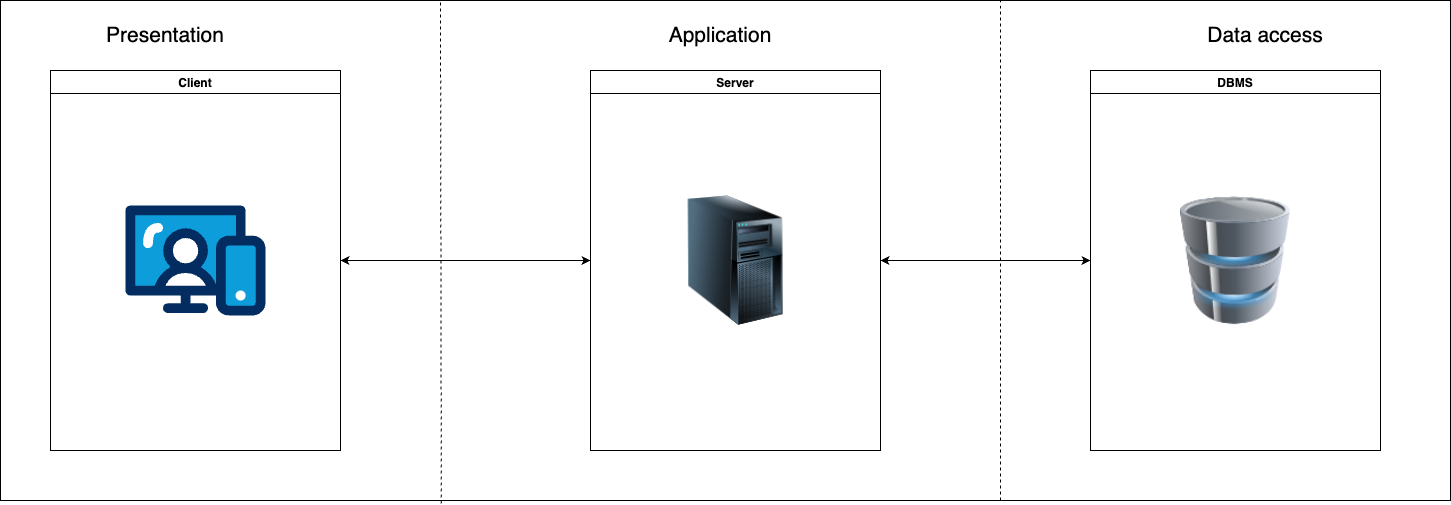
\includegraphics[width=\textwidth]{Images/three_tier.png}
    \caption{High level components and their interaction}
\end{figure}

The three-tier architecture was chosen for this type of system because of the several advantages it offers compared to other types of architectures. For what concerns scalability, it allows for easy scalability by separating the presentation, application, and data layers. Each layer can be scaled independently, allowing for better performance and resource utilization.
For what concers modulatiry, it promotes the separation of concers by dividing the system into distinct layers. This makes it easier to develop, test, and maintain each layer separately, improving overall code quality and reusability. The sepatarion of concerns also improves the maintainability of the system by providing clear boundaries between layers it makes easier to understand and modify specific parts of the system without affecting other layers.
The last advantage for which this architecture was chosen is flexibility. The three-tier provides flexibility in terms of technology choices. Each layer can be implemented using different technologies, allowing for the use of the most suitable tools and frameworks for each specific layer.

\begin{figure}[H]
    \centering
    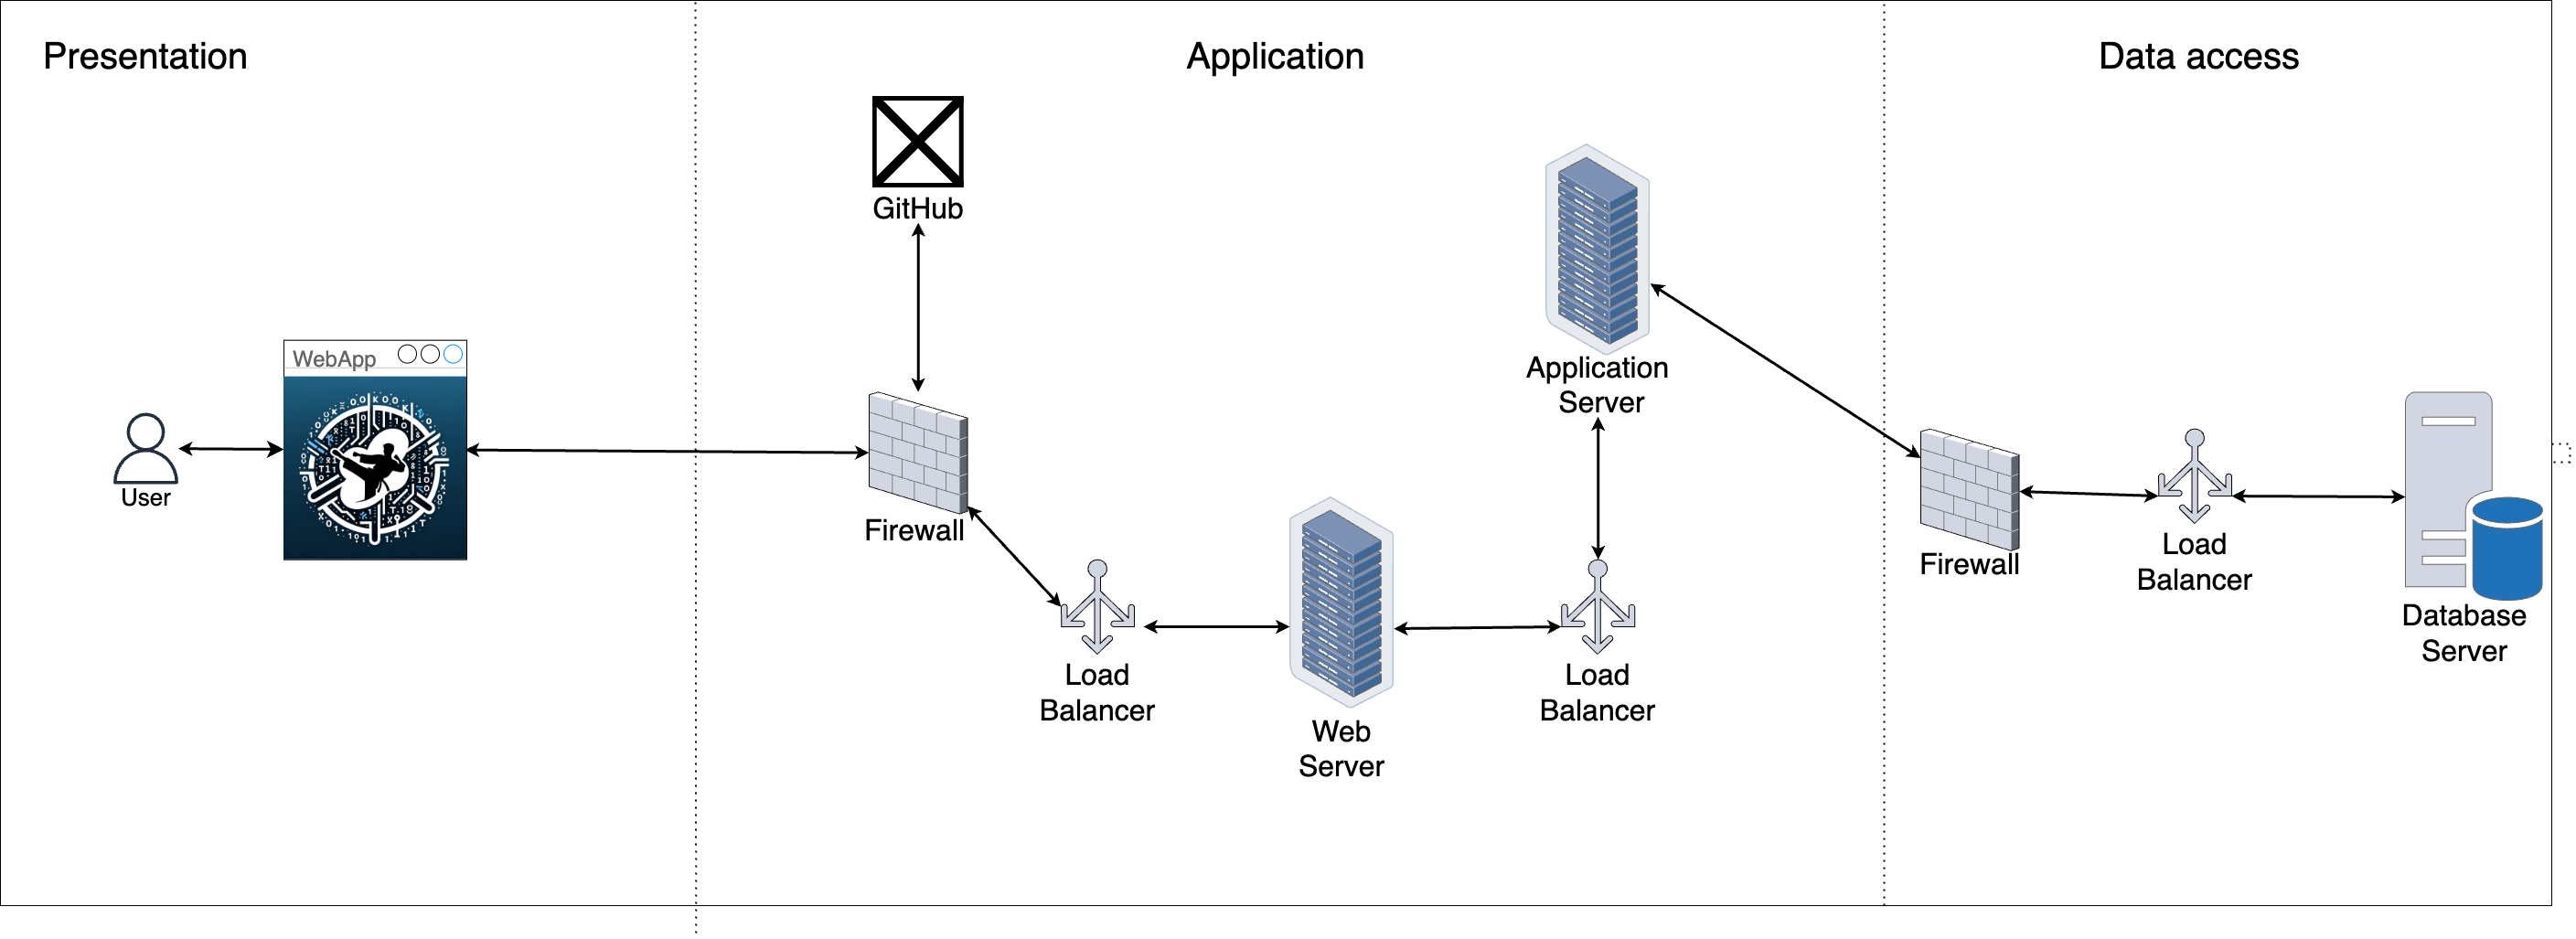
\includegraphics[width=\textwidth]{Images/high_level.png}
    \caption{High level system with interactions between the components}
    \label{fig:high_level_system}
\end{figure}

In the figure Figure\ \ref{fig:high_level_system} is shown the high level system with the interactions between the components. 
At the forefront is the Presentation layer, where a user engages with the web application through a web browser.
The web application depending on user interactions requests data from the web server. The interaction between the two is not direct since there is a firewall (for security reasons) and also a load balancer.

Moving inward, the Application layer serves as the system's operational core, where a network firewall establishes the first line of defense, safeguarding the internal processes. A load balancer stands right behind the firewall, directing incoming traffic to maintain system efficiency and reliability. This layer is further composed by an application server that executes the business logic, interfacing with databases or other external services as needed. Additionally, the presence of an upward arrow connecting the load balancer to GitHub to handle the evaluation trigger as well as the creation of the repositories. This is a very important feature of the system since it allows to automatically evaluate the students' submissions.

The final segment of the diagram is the Data Access layer, echoing the security and balance themes with its own firewall and load balancer, underscoring the system's commitment to secure data transactions. At the heart of this layer lies the database server, a robust storage solution that ensures data is efficiently stored, retrieved, and managed, completing the architecture's promise of a secure, scalable, and resilient web application environment.

\subsection{Component view}
In Figure\ \ref{fig:component_diagram} is shown the component diagram of the system. The system is divided into three main layers: presentation layer, application layer and data layer. The presentation layer is the interface between the user and the system and it is represented with the WebApp and Web Server Component. The application layer is the core of the CKB Platform and it is representend by the Application Server Subsystem. Finally the data layer is represented by the DBMS Component who is the only one that access the database.
\begin{figure}[H]
    \centering
    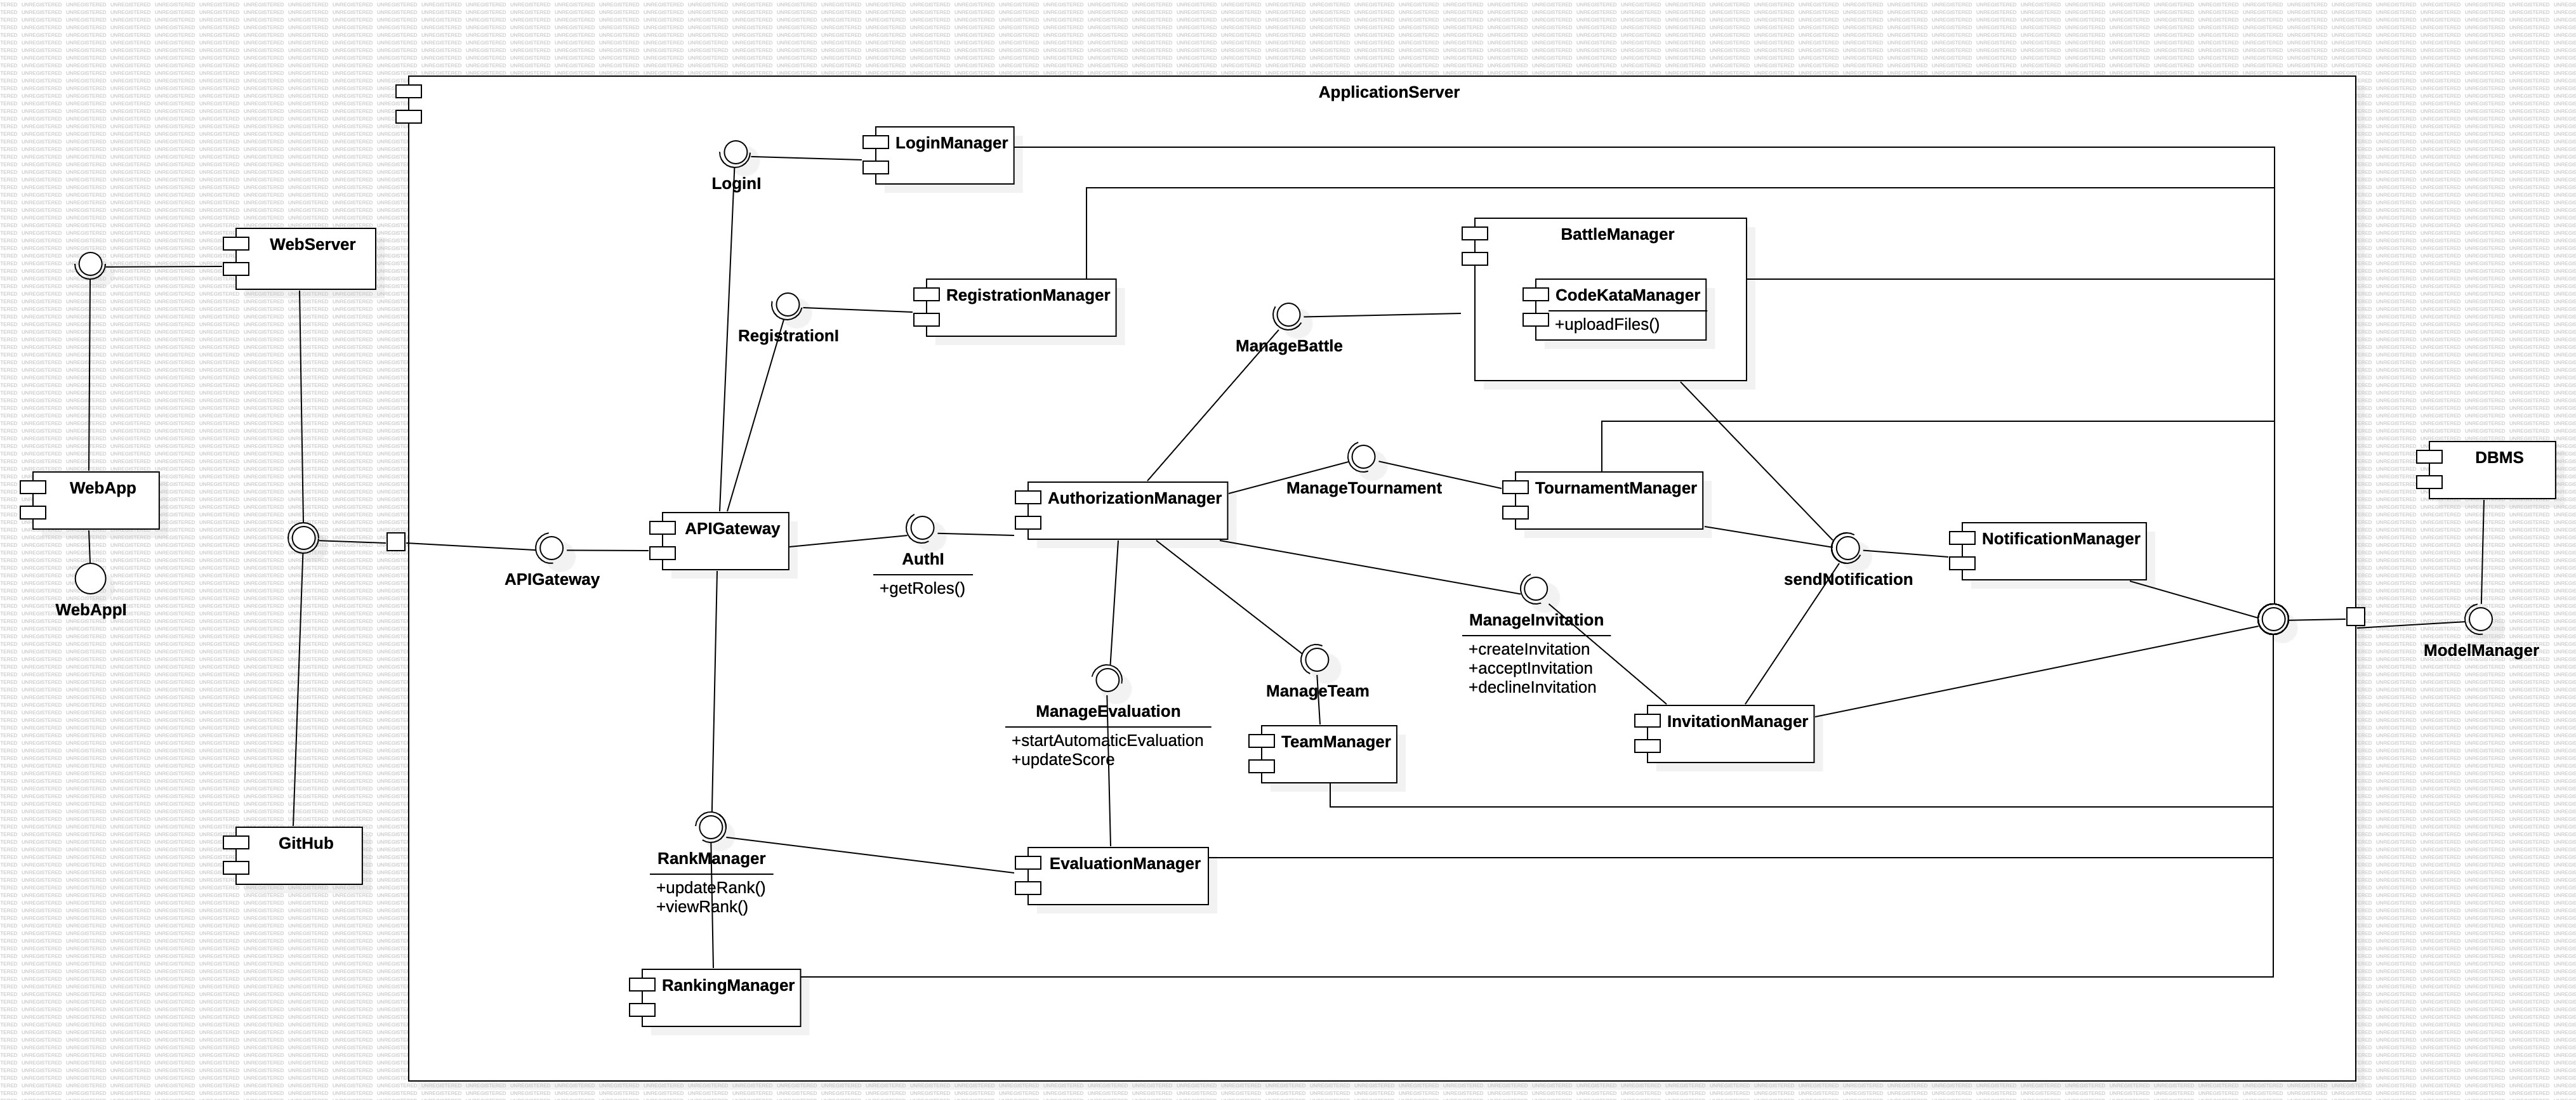
\includegraphics[angle=90,origin=c,width=0.6\textwidth]{Diagrams/ComponentDiagram.jpg}
    \caption{Component diagram}
    \label{fig:component_diagram}
\end{figure}
\clearpage
Regarding the presentation layer, it is represented by the following two components:
\begin{itemize}
    \item \textbf{WebApp}: it is the web application that the user interacts with. It is responsible for the presentation of the data and the interaction with the user. Since it communicates only with the Web Server, it can be executed by any device that has a web browser.
    \item \textbf{Web Server}: it is the component that handles the requests from the WebApp and forwards them to the Application Server. It is responsible to direct the requests to the APIGateway. It is also responsible to forward responses from the Application Server to the WebApp.
\end{itemize}
Regarding the application layer, it is represented by the components inside the Application Server Subsystem:
\begin{itemize}
    \item \textbf{APIGateway}: it is the component that handles the incoming requests to the Application Server. It is responsible to direct the requests to the correct component inside the Application Server Subsystem. It is also responsible to forward responses from the Application Server to the Web Server.
    \item \textbf{Login Manager}: it is the component that handles the login requests. It is responsible to check the credentials and to log the user in.
    \item \textbf{Registration Manager}: it is the component that handles the registration requests. It is responsible to create a new user.
    \item \textbf{Authorization Manager}: it is the component that handles the authorization requests. It is responsible to check if the user is authorized to perform the requested action. This is of paramount importance since only a user with Educator role can perform administrative actions, such as the creation of a new Tournament or Battle.
    \item \textbf{Evaluation Manager}: it is the component that handles the evaluation requests. It is responsible to evaluate the submissions of the students and to return the results. It performs the evaluation by running and testing the submissions provided by the students. It can be used also by the Educator to re-evaluate the submissions manually.
    \item \textbf{Ranking Manager}: it is the component that handles the rank of students in a Tournament.
    \item \textbf{Team Manager}: it is the component that handles the creation of teams and the assignment of students to teams. It is also responsible to guarantee that the restrictions on the number of students per team, set by the Educator, are respected.
    \item \textbf{Submission Manager}: it is the component that handles the submission of the students. The submission is created when the GitHub Action is triggered by the push of the student in the Team repository. It interacts with the Evaluation Manager to get the evaluation of the submission.
    \item \textbf{Invitation Manager}: it is the component that handles the invitation of both Students and Educator. In the case of the Students it is responsible to manage the invitation to join a Team. In the case of the Educator it is responsible to manage the invitation to join a Tournament.
    \item \textbf{Notification Manager}: it is the component that handles the notification requests. It is responsible to send notifications to the users. Such notifications are sent respecting the conditions previously specified in the RASD document.
    \item \textbf{Battle Manager}: it is the component that handles the creation and the management of Battles by the Educator. It is a complex component since it embodies also the CodeKata Manager. Since it contains the CodeKata Manager, it is responsible to handle the CodeKata files uploaded by the Educator. It interacts with the GitHub Component to create the repositories for the Battles. It also handles the different Battle phases, by guaranteeing the deadline restrictions set by the Educator.
    \item \textbf{Tournament Manager}: it is the component that handles the creation and the management of Tournaments by the Educator. It is responsible to handle the different Tournament phases, by guaranteeing the deadline restrictions set by the Educator.
\end{itemize}
Regarding the data layer, it is represented by the following component:
\begin{itemize}
    \item \textbf{DBMS}: it is the component that handles the access to the database. It is responsible to store and retrieve the data from the database. It is the only component that can access the database.
\end{itemize}
\subsection{Deployment view}
In this section is shown the deployment diagram of the system. The diagram is divided into three main tier: the presentation tier, the application tier and the data tier. 
\begin{figure}[H]
    \centering
    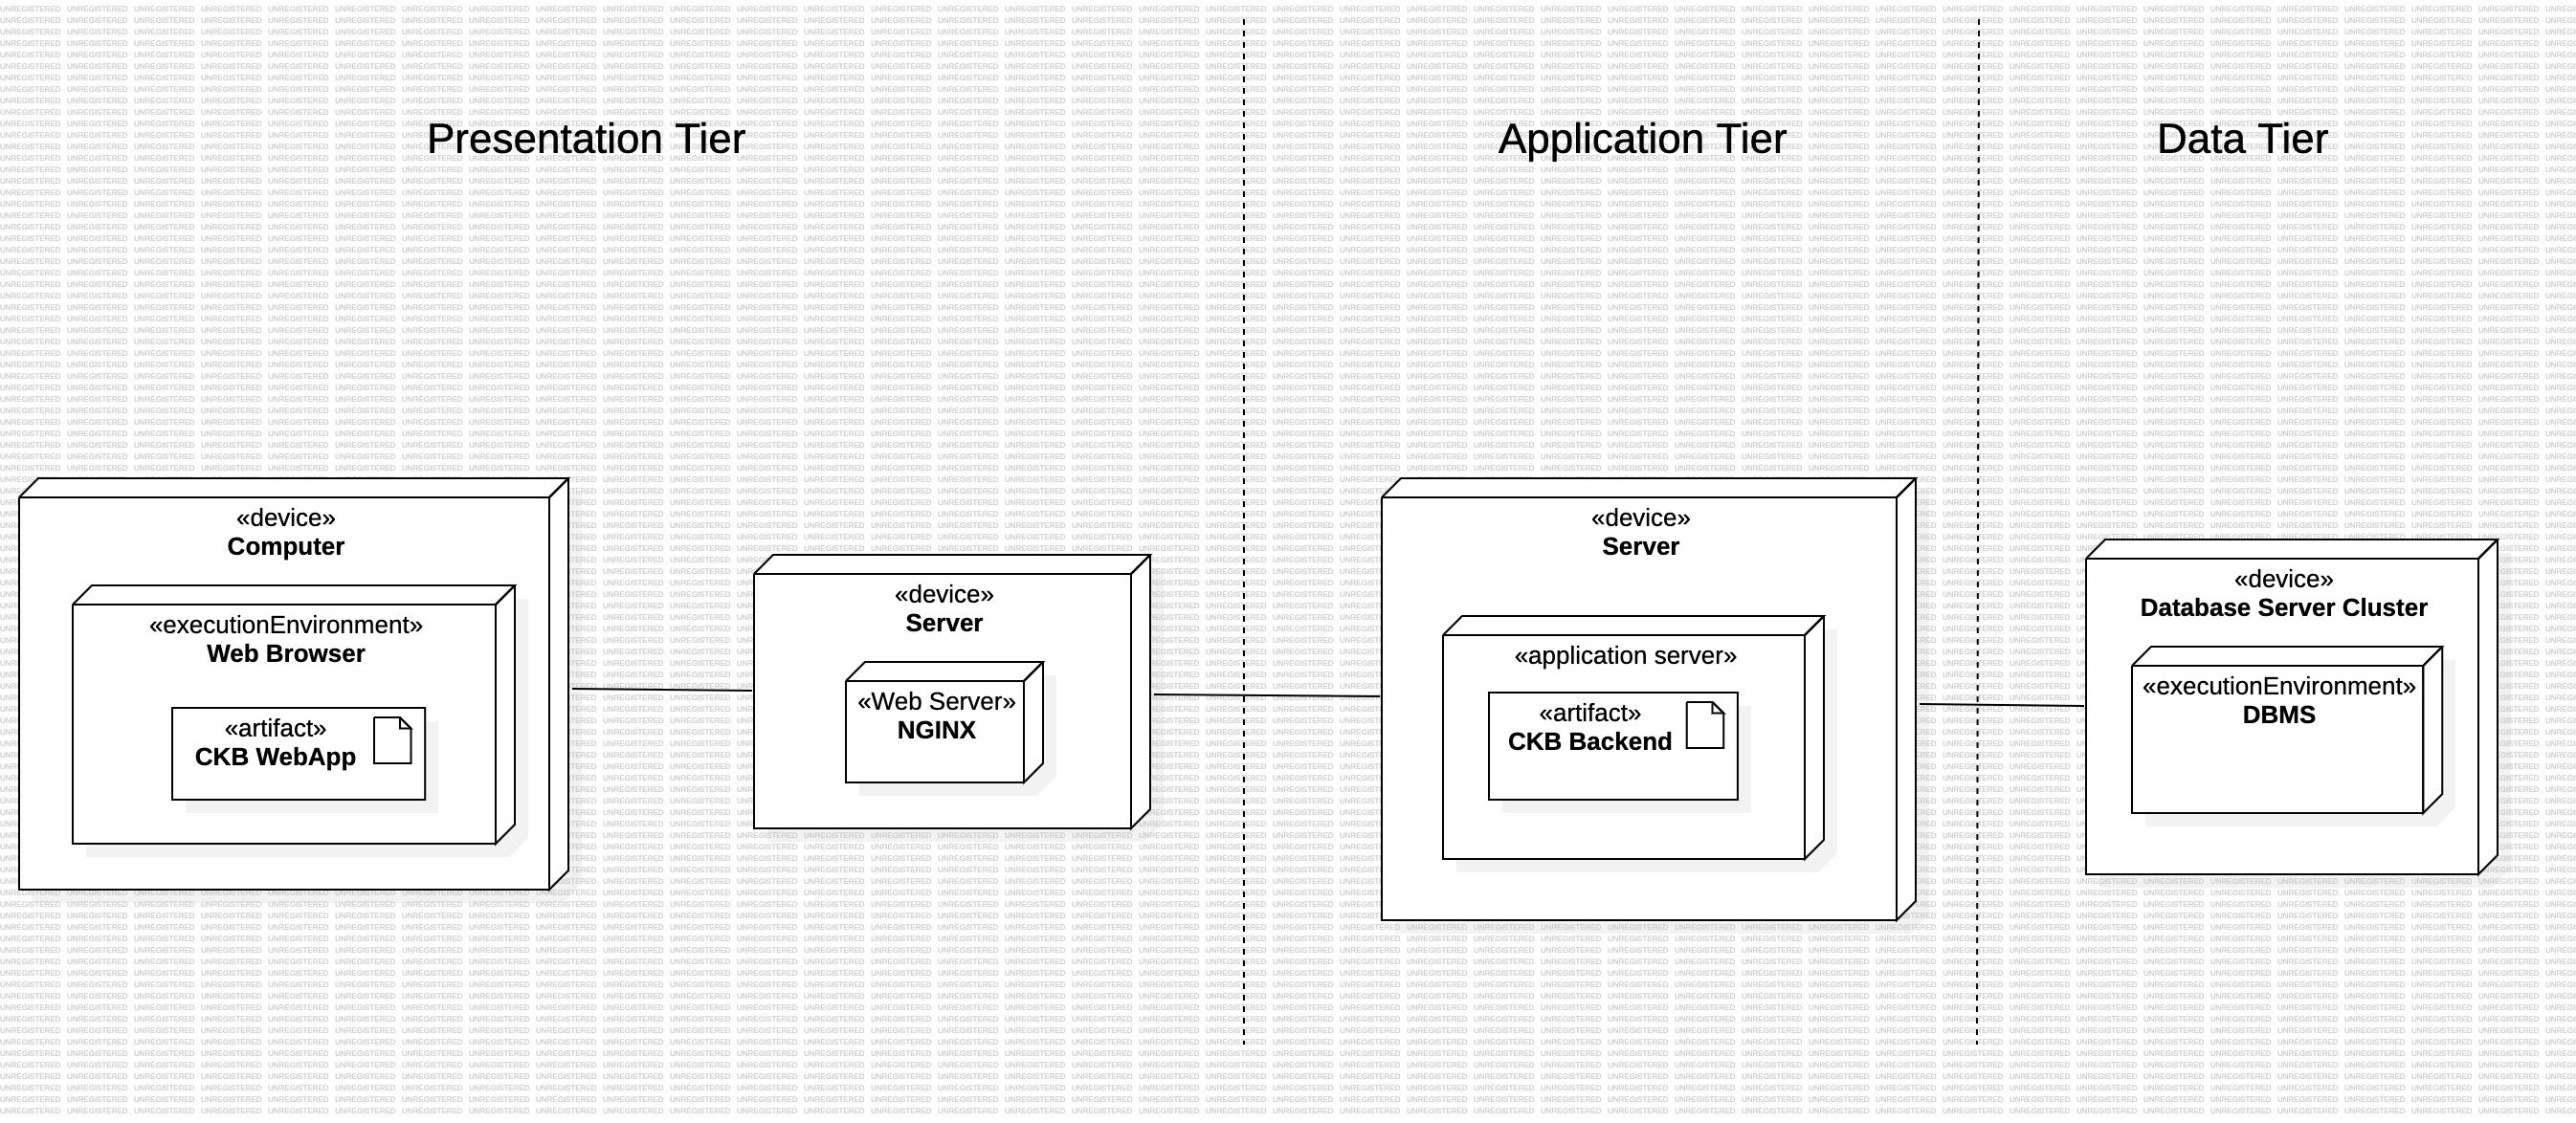
\includegraphics[width=\textwidth]{Diagrams/DeploymentDiagram.jpg}
    \caption{Deployment diagram}
    \label{fig:deployment_diagram}
\end{figure}
In figure Figure\ \ref{fig:deployment_diagram} is shown the deployment diagram of the system.
Regarding the presentation tier, it is represented by the following components:
\begin{itemize}
    \item \textbf{Computer}: it is a normal computer used by the user. It is the device that the user uses to interact with the CKB WebApp. It has no particular requirements since it only needs a web browser to access the WebApp.
    \item \textbf{Web Browser}: it is the software that the user uses to interact with the CKB WebApp. The CKB platform has to support the most common web browsers, such as Google Chrome, Mozilla Firefox, Microsoft Edge and Apple Safari.
    \item \textbf{CKB WebApp}: it is the web application that the user interacts with and it is used within the web browser. It is responsible for the presentation of the data and the interaction with the user.
    \item \textbf{Web Server}: it is a server that hosts a NGINX web server instance. The choice of NGINX is due to its high performance, low memory usage and high availability.
\end{itemize}
Regarding the application tier, it is represented by the following components:
\begin{itemize}
    \item \textbf{Application Server}: it is a server that hosts a CKB Backend application instance. It receives the requests from the Web Server and forwards it to the CKB Backend. At the same time it provides responses to the Web Server. It is also responsible to communicate with the DBMS to retrieve and store data.
    \item \textbf{CKB Backend}: it is the backend application of the CKB Platform. It handle the entire business logic of the application. It is responsible to process the forwarded requests and to provide responses to the Application Server.
\end{itemize}
Regarding the data tier, it is represented by the following components:
\begin{itemize}
    \item \textbf{Database Server Cluster}: it is a cluster of servers that hosts a DBMS instance. The choice of a cluster is due to the fact that it provides high availability and scalability. It is also responsible to guarantee the security of the data. It process the database specific requests sent by the Application Server.
    \item \textbf{DBMS}: it is the software that manages the database. It is responsible to store and retrieve the data from the database. It is the only component that can access the database.
\end{itemize}
\subsection{Component interfaces}

\textbf{Interface} LoginManager:
\begin{itemize}
    \item \texttt{Session login(String username, String password);}
    \item \texttt{void logout(Session session);}
\end{itemize}

\textbf{Interface} RegistrationManager:
\begin{itemize}
    \item \texttt{boolean register(UserDetails userDetails);}
\end{itemize}

\textbf{Interface} AuthorizationManager:
\begin{itemize}
    \item \texttt{List<Role> getRoles(User user);}
    \\ Get the roles of a user. The roles are used to determine if a user is authorized to perform a specific action.
\end{itemize}

\textbf{Interface} BattleManager:
\begin{itemize}
    \item \texttt{Battle createBattle(BattleDetails details);}
    \\ Create a new Battle. The BattleDetails contains all the information needed to create a new Battle.
    \item \texttt{boolean uploadFiles(Battle battle, CodeKata files);}
    \\ Upload the files of the CodeKata. The files must contain the tests and the automation scripts of the CodeKata.
    \item \texttt{boolean updateBattle(Battle battle, BattleDetails details);}
    Updates the details of a Battle, such as the different stages and the deadlines.
    \item \texttt{List<Team> getTeams(Battle battle);}
\end{itemize}

\textbf{Interface} TournamentManager:
\begin{itemize}
    \item \texttt{Tournament createTournament(TournamentDetails details);}
    \\ Create a new Tournament. The TournamentDetails contains all the information needed to create a new Tournament.
    \item \texttt{boolean updateTournament(Tournament tournament, TournamentDetails details);}
    \\ Updates the details of a Tournament, such as the different stages and the deadlines.
\end{itemize}

\textbf{Interface} InvitationManager:
\begin{itemize}
    \item \texttt{boolean sendInvitation(User user, Invitation invitation);}
    \\ Send an invitation to a user. The invitation can be to join a Tournament, if the user is an Educator, or to join a Team, if the user is a Student.
    \item \texttt{boolean acceptInvitation(Invitation invitation);}
    \\ Accept an invitation sent by another user.
    \item \texttt{boolean declineInvitation(Invitation invitation);}
    \\ Decline an invitation sent by another user.
\end{itemize}

\textbf{Interface} RankingManager:
\begin{itemize}
    \item \texttt{void updateRank(Student student, Tournament tournament, int newRank);}
    \\ Update the rank of a Student in a Tournament. This method can only be used by users with Educator Role.
    \item \texttt{int viewRank(Student student, Tournament tournament);}
    \\ View the rank of a Student in a Tournament.
\end{itemize}

\textbf{Interface} SubmissionManager:
\begin{itemize}
    \item \texttt{SubmissionResult submit(Item item);}
    \\ Submit a solution to a Battle. The Item contains the code of the solution. The SubmissionResult contains the evaluation of the submission.
    \item \texttt{Item getSubmission(int submissionId);}
    \\ Get the code of a submission given its id.
    \item \texttt{SubmissionResult getSubmissionResult(int submissionId);}
    \\ Get the evaluation of a submission given its id.
\end{itemize}

\textbf{Interface} NotificationManager:
\begin{itemize}
    \item \texttt{void notify(User user, Notification notification);}
    \\ Send a notification to a user.
\end{itemize}

\textbf{Interface} ModelManager:
\begin{itemize}
    \item \texttt{boolean saveModel(DataModel model);}
    \\ Save a DataModel in the database.
    \item \texttt{DataModel getModel(DataModel model, List<Filter> filters);}
    \\ Get a DataModel from the database given its id.
    \item \texttt{boolean updateModel(DataModel model);}
    \\ Update a DataModel in the database.
    \item \texttt{boolean deleteModel(DataModel model);}
    \\ Delete a DataModel from the database.
\end{itemize}

\textbf{Interface} TeamManager:
\begin{itemize}
    \item \texttt{Team createTeam(TeamDetails details);}
    \\ Create a new Team. The TeamDetails contains all the information needed to create a new Team.
    \item \texttt{boolean updateTeam(Team team, TeamDetails details);}
    \\ Updates the details of a Team, such as the name and the members.
    \item \texttt{boolean addMember(Team team, Student student);}
    \\ Add a Student to a Team.
\end{itemize}
\subsection{Runtime view}
In this section are shown the sequence diagrams of the main functionalities of the system previously described in the RASD document. Starting from the \textit{Component View} section of this document, it is possible to identify the components interactions that are shown in the following sequence diagrams.
\subsubsection*{Login}
\begin{figure}[H]
    \centering
    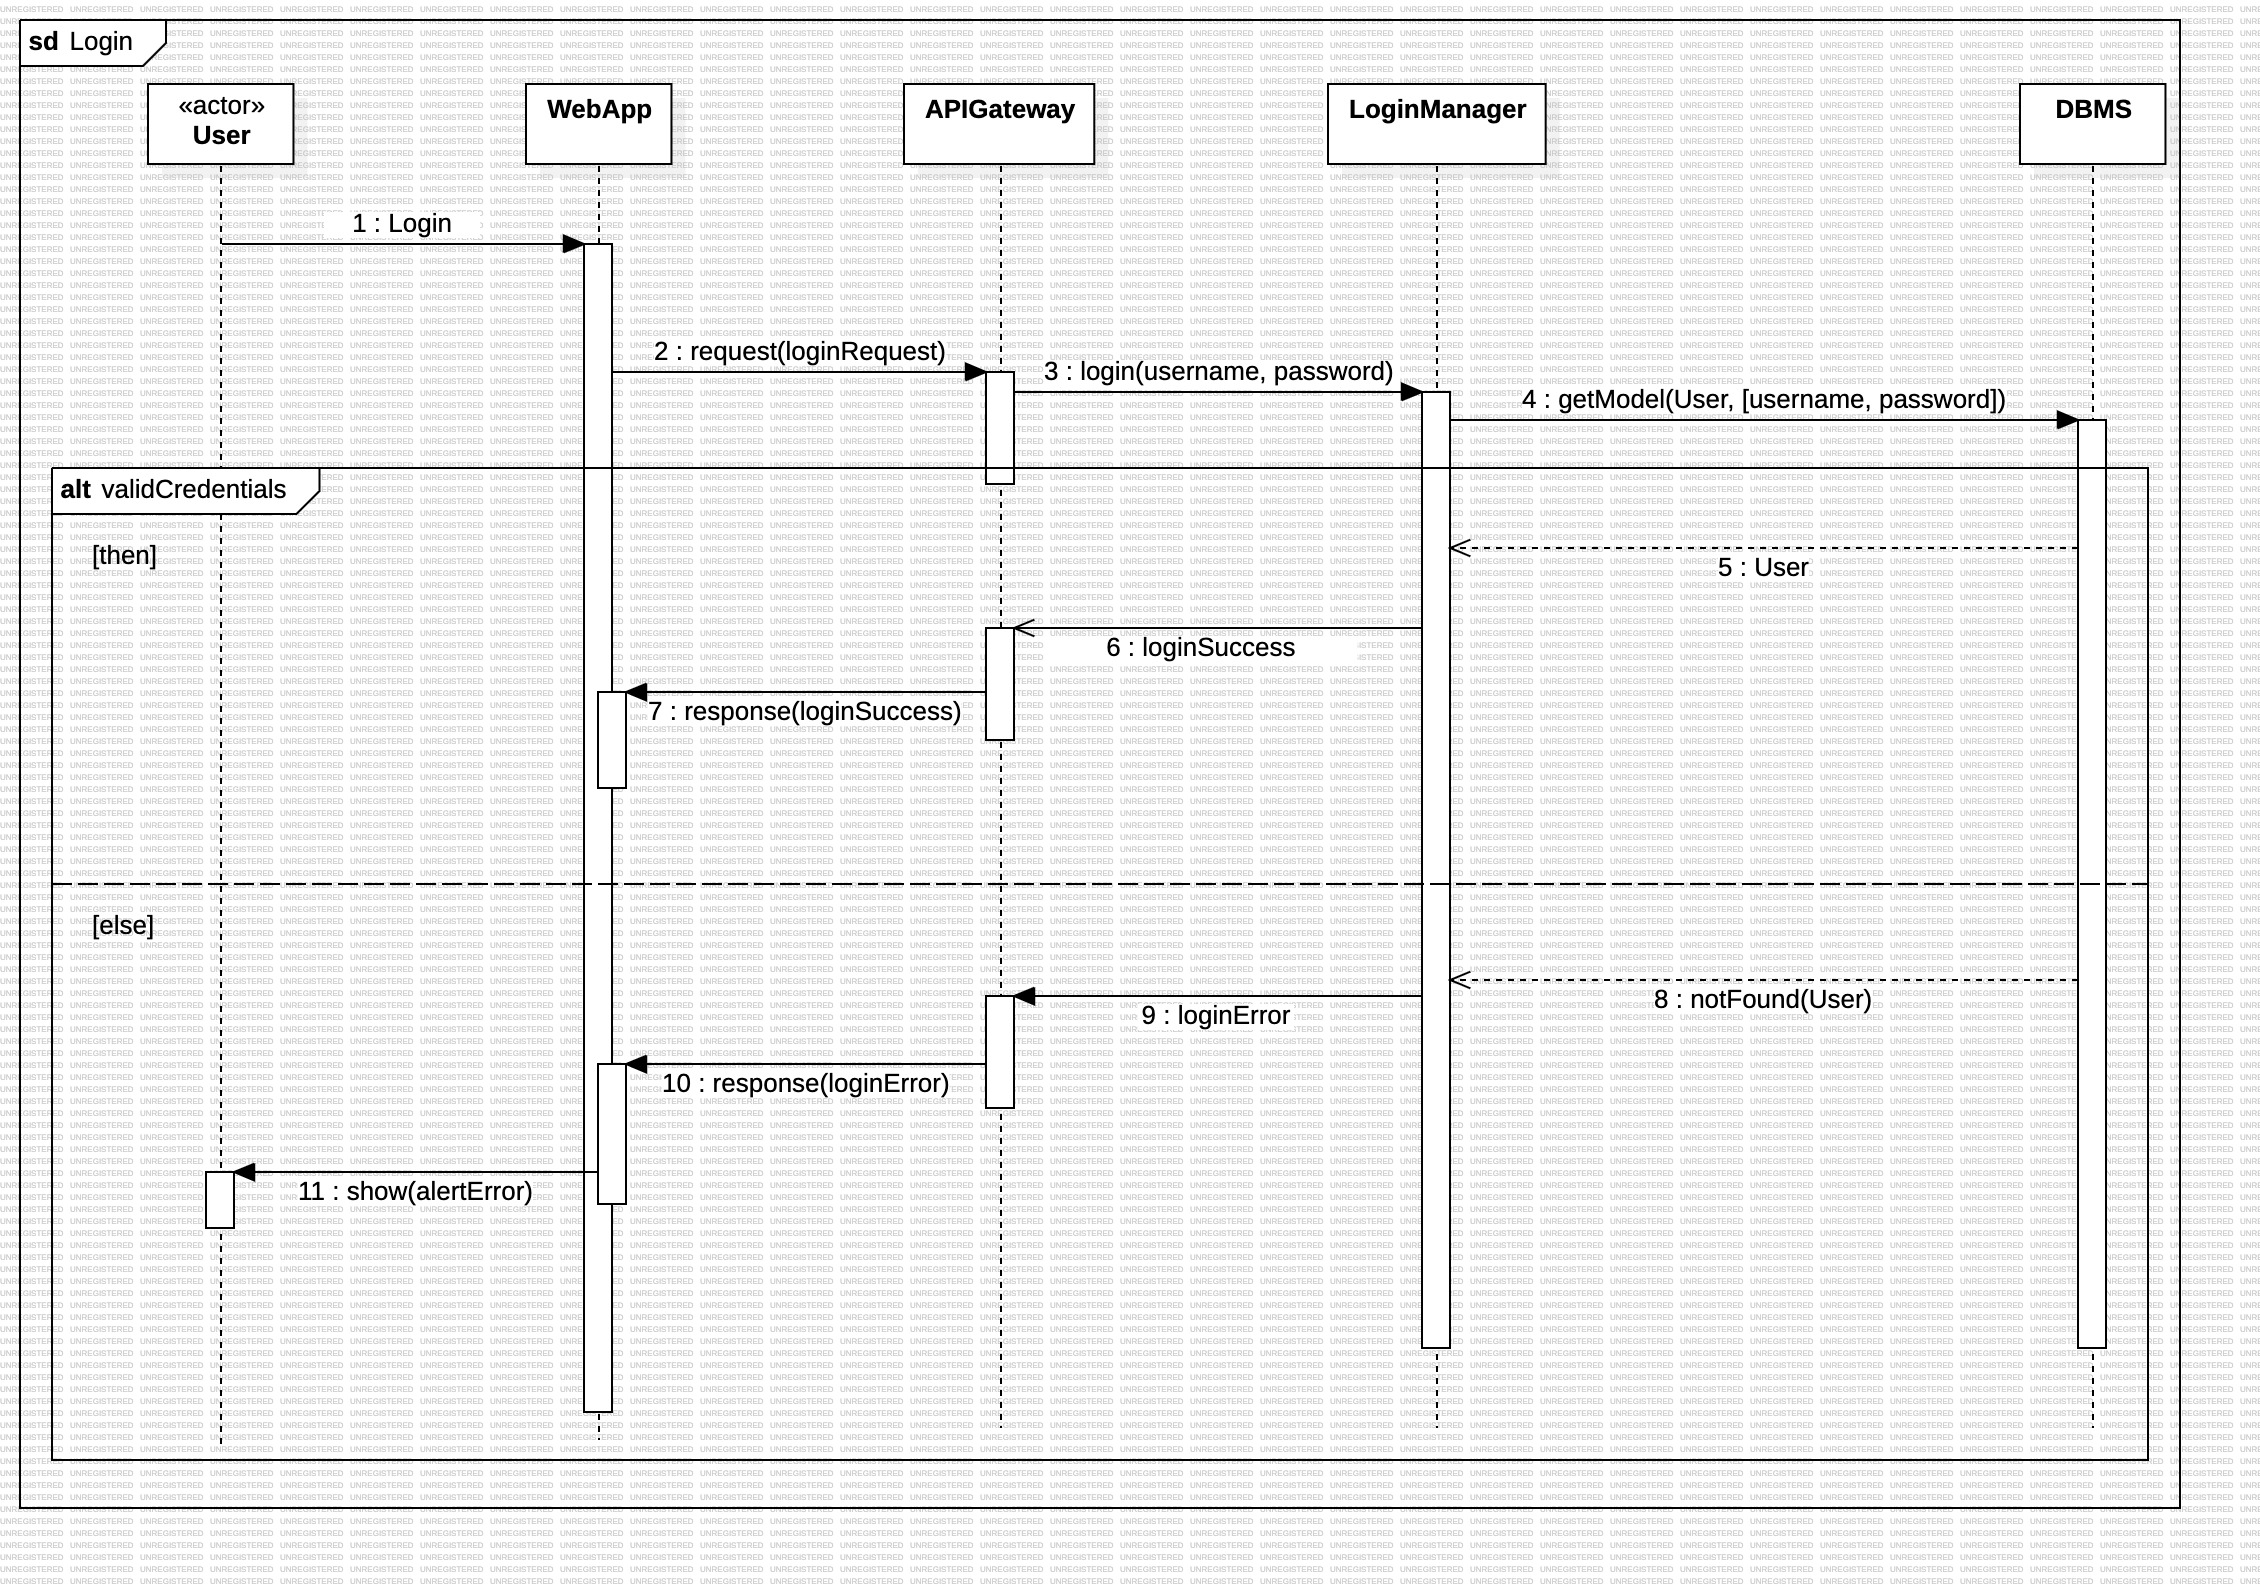
\includegraphics[width=\textwidth]{Diagrams/LoginSD.jpg}
    \caption{Runtime view}
    \label{fig:runtime_view}
\end{figure}
\subsection{Selected architectural styles and patterns}
\subsubsection{Three-tier architecture}
The three-tier architecture offers several key advantages of paramount importance for the CKB Platform:
\begin{enumerate}
    \item \textbf{Scalability}: by separating concerns into different layers, it becomes easier to scale each tier independently based on demand.
    \item \textbf{Maintainability}: modifications in one tier can be implemented without impacting the other tiers, simplifying maintenance and updates.
    \item \textbf{Flexibility}: Each tier can utilize the most suitable technologies, allowing for technological adaptability. For example: the presentation layer can adopt a frontend framework that best suits the needs of the application, while the application layer can adopt a backend framework that best suits the needs of the application.
    \item \textbf{Security}: Layer separation enables specific security measures at each level, enhancing overall protection. In the Figure\ \ref{fig:high_level_system} is shown that the different tier are physically connected through firewalls. This is a very important feature of the system since it allows to guarantee the security of the data.
    \item \textbf{Easier Testing and Debugging}: Individual layer testing and debugging lead to more efficient problem resolution. Different teams can work on different layers simultaneously, allowing for faster testing and debugging.
    \item \textbf{Improved Performance}: Effective load balancing across layers results in better overall system performance.
\end{enumerate}
\subsubsection{Model View Controller (MVC) pattern}
The Model-View-Controller (MVC) pattern is a software design paradigm that organizes an application into three interconnected components:

\begin{itemize}
    \item \textbf{Model:} Manages the data and business logic of the application.
    \item \textbf{View:} Responsible for the display and user interface.
    \item \textbf{Controller:} Acts as an intermediary between the Model and View, processing user input and responding to user interactions.
\end{itemize}
The MVC pattern is a good fit for the CKB Platform because as discussed above the platform is decomposed into three layer. In particular: the \textit{Model} is represented by the DBMS Component, the \textit{View} is represented by the WebApp Component and the WebServer subsystem. Finally the \textit{Controller} is represented by the Application Server Subsystem which implement several components such as the Login Manager, the Registration Manager, the Authorization Manager, the Evaluation Manager, the Ranking Manager, the Team Manager, the Submission Manager, the Invitation Manager, the Notification Manager, the Battle Manager and the Tournament Manager that are responsible to handle the data, process following the business logic and pass it to the \textit{View}. \\
Some of the benefits apported by the MVC to the CKB Platform are:

\begin{enumerate}
    \item \textbf{Modularity:} Separation of concerns allows for independent development, maintenance, and testing of each component.
    \item \textbf{Reusability:} Facilitates the reuse of components, especially the business logic encapsulated in the Model.
    \item \textbf{Scalability:} Makes scaling and updating the application more manageable as it grows in complexity.
    \item \textbf{Flexibility:} Each component can evolve independently, accommodating new technologies or changes in business requirements.
    \item \textbf{Improved Organization:} Enhances code readability and maintainability due to its structured organization.
    \item \textbf{Simplified Collaboration:} Enables different development teams to work on each component without overlap, improving collaborative efforts.
\end{enumerate}

\subsubsection{Facade pattern}
\subsubsection{Observer pattern}
\subsection{Other design decisions}


%------------------------------------------------------------------------------------------------------------------------------------------------
\clearpage
{\color{Blue}{\section{User Interface Design}}}
\label{sect:userInterfaceDesign}

\begin{figure}[H]
    \centering
    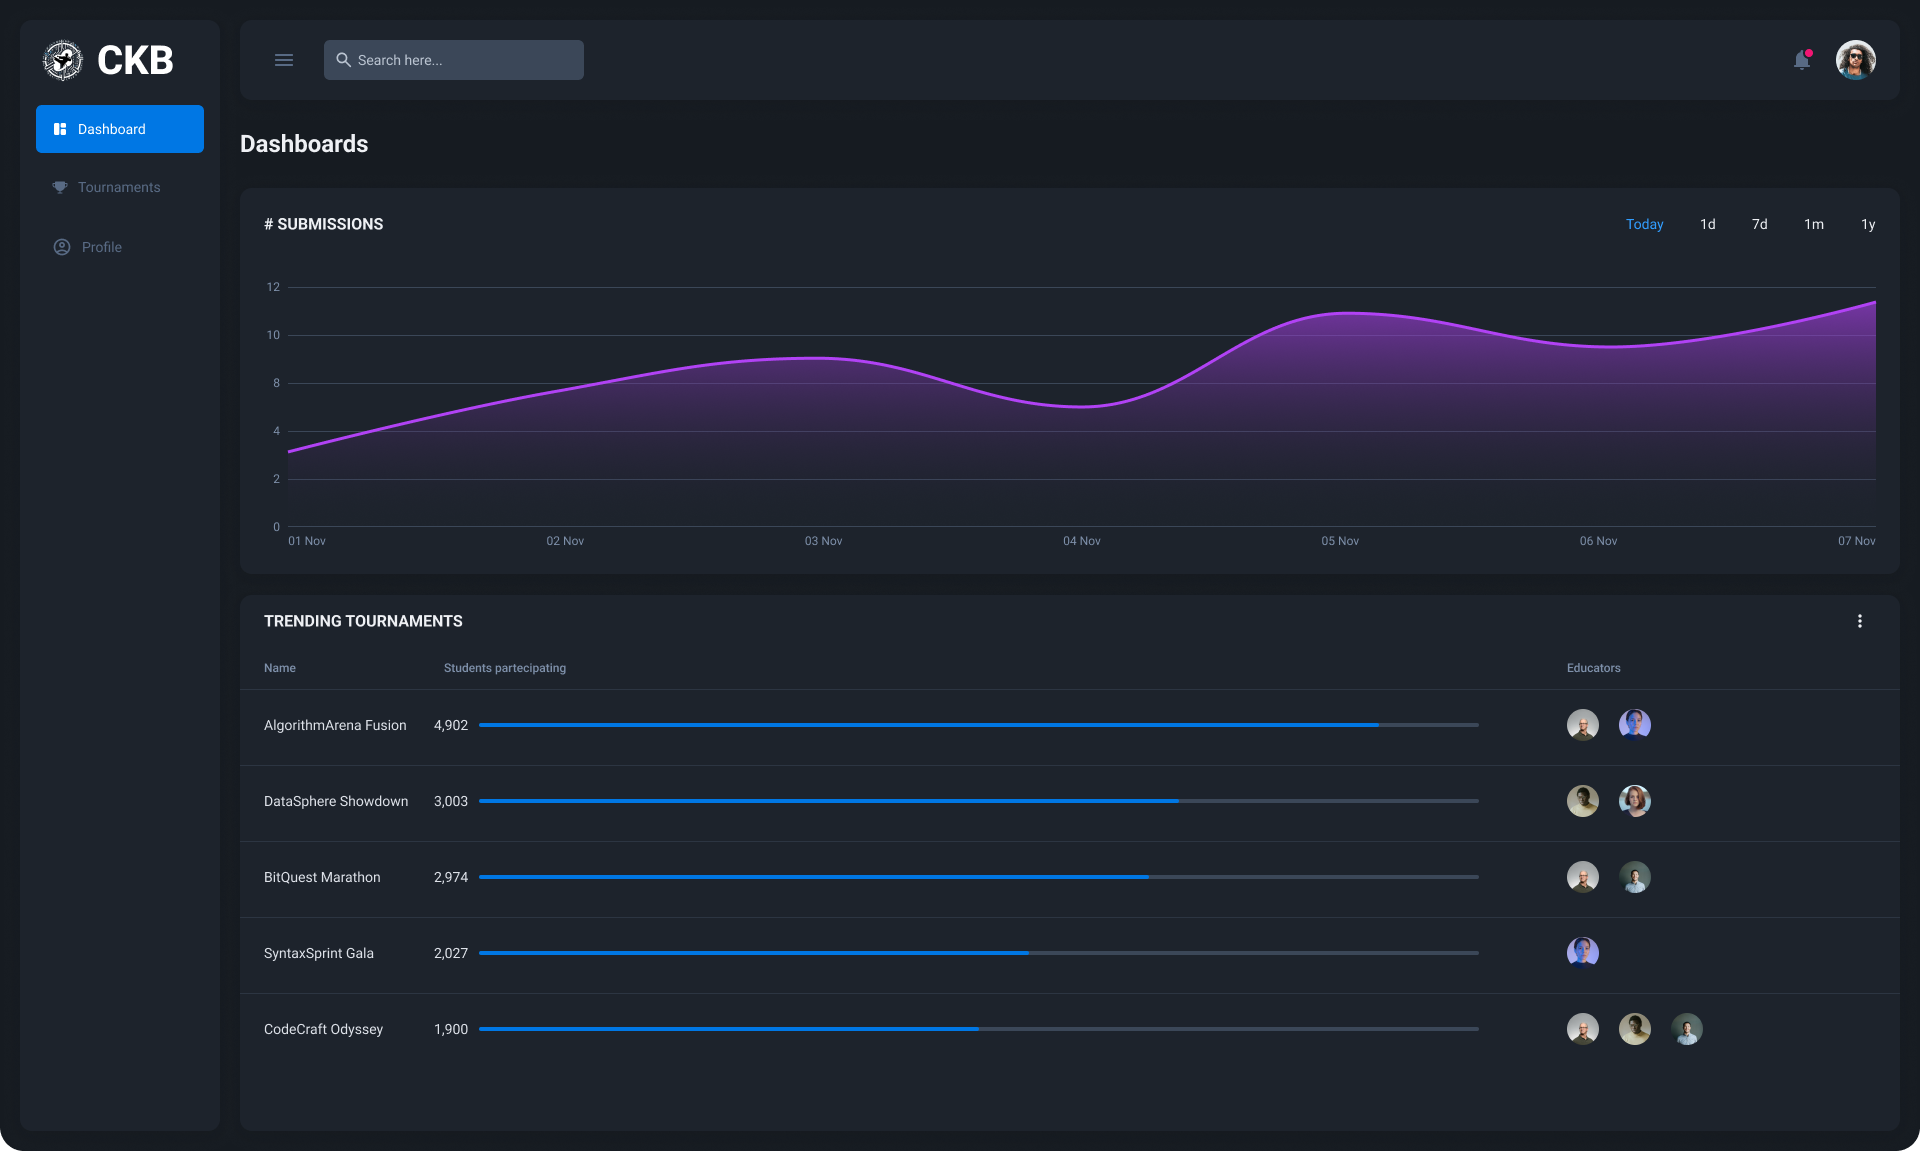
\includegraphics[width=\textwidth]{Images/Dashboard-Student.png}
    \caption{Student Dashboard}
    \label{fig:student-dashboard}
\end{figure}

\begin{figure}[H]
    \centering
    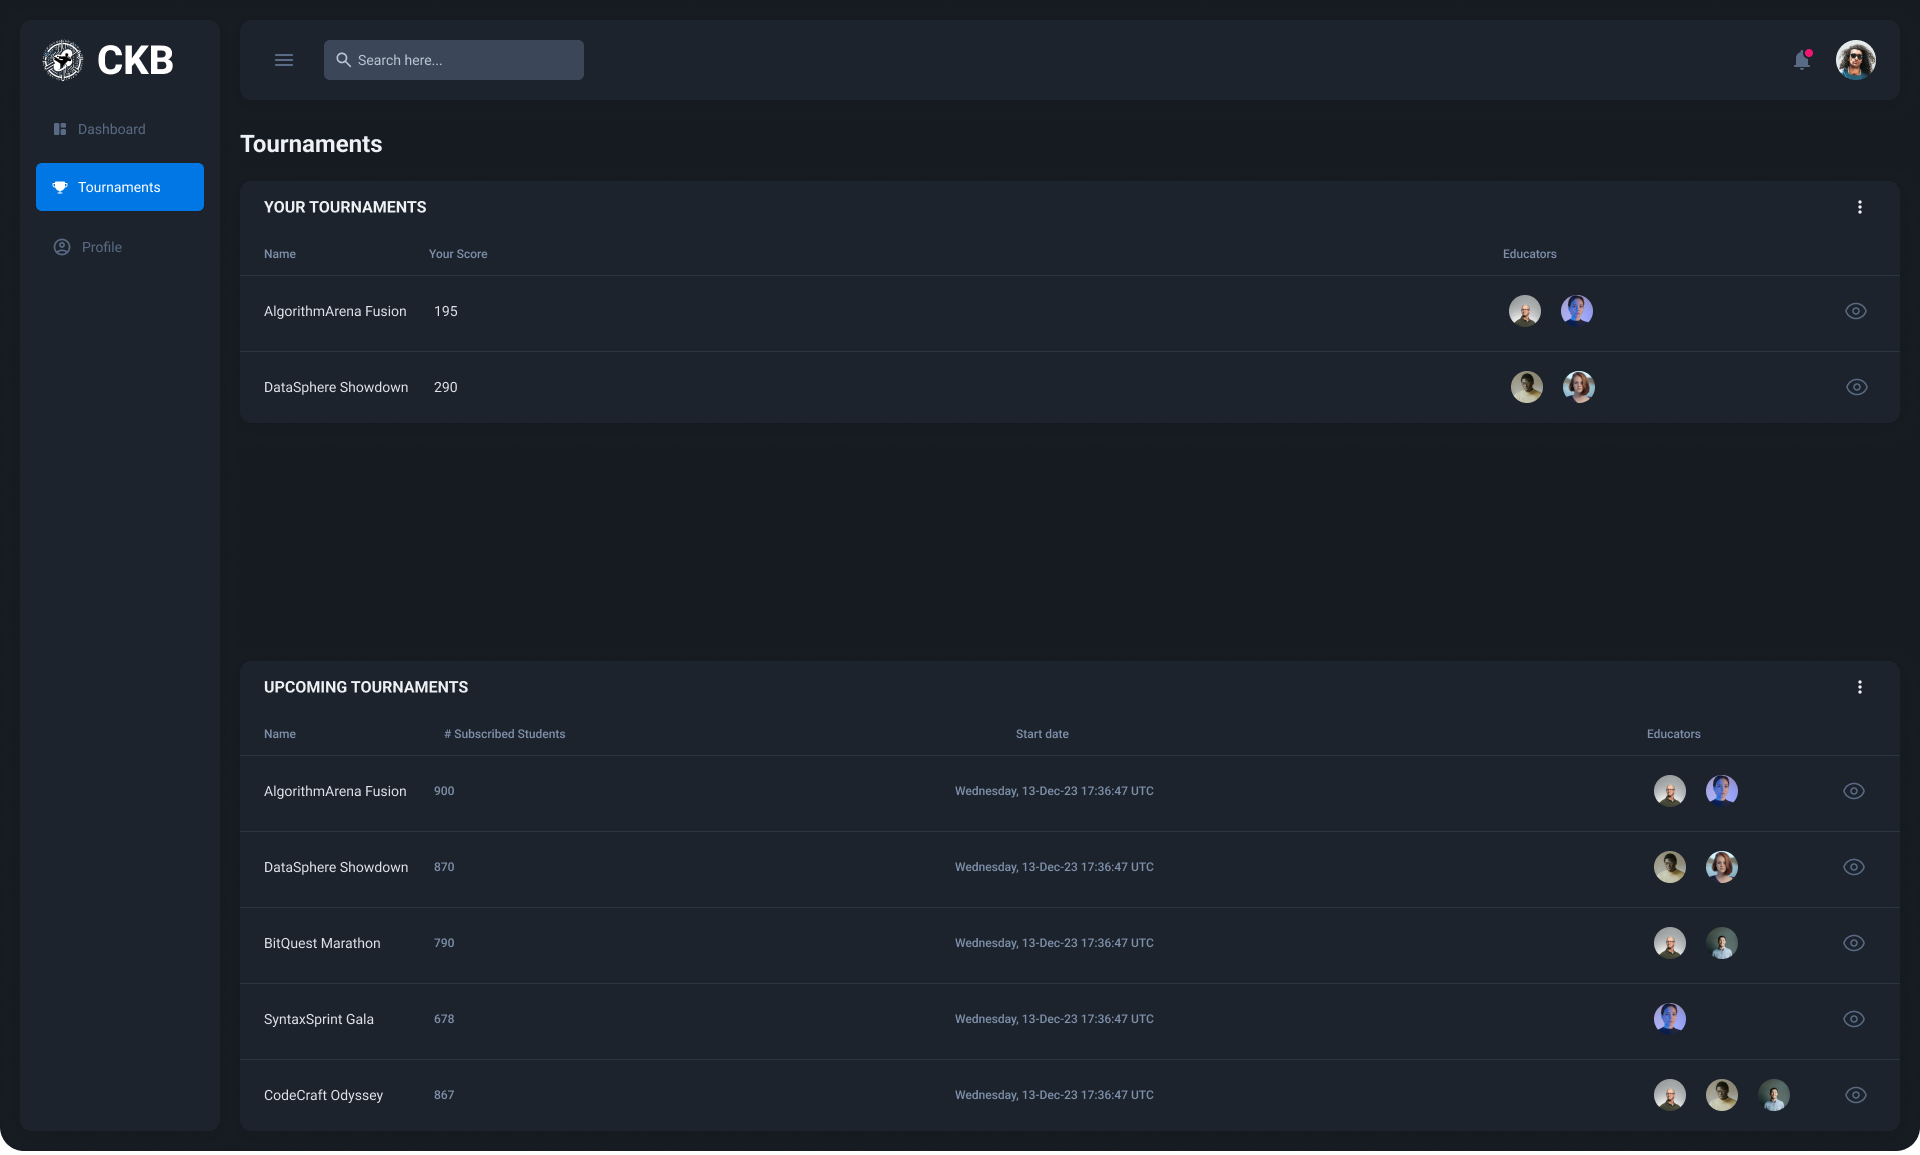
\includegraphics[width=\textwidth]{Images/Dashboard-Tournament.png}
    \caption{Student Dashboard Tournaments Tab}
    \label{fig:student-dashboard-tournaments}
\end{figure}

\begin{figure}[H]
    \centering
    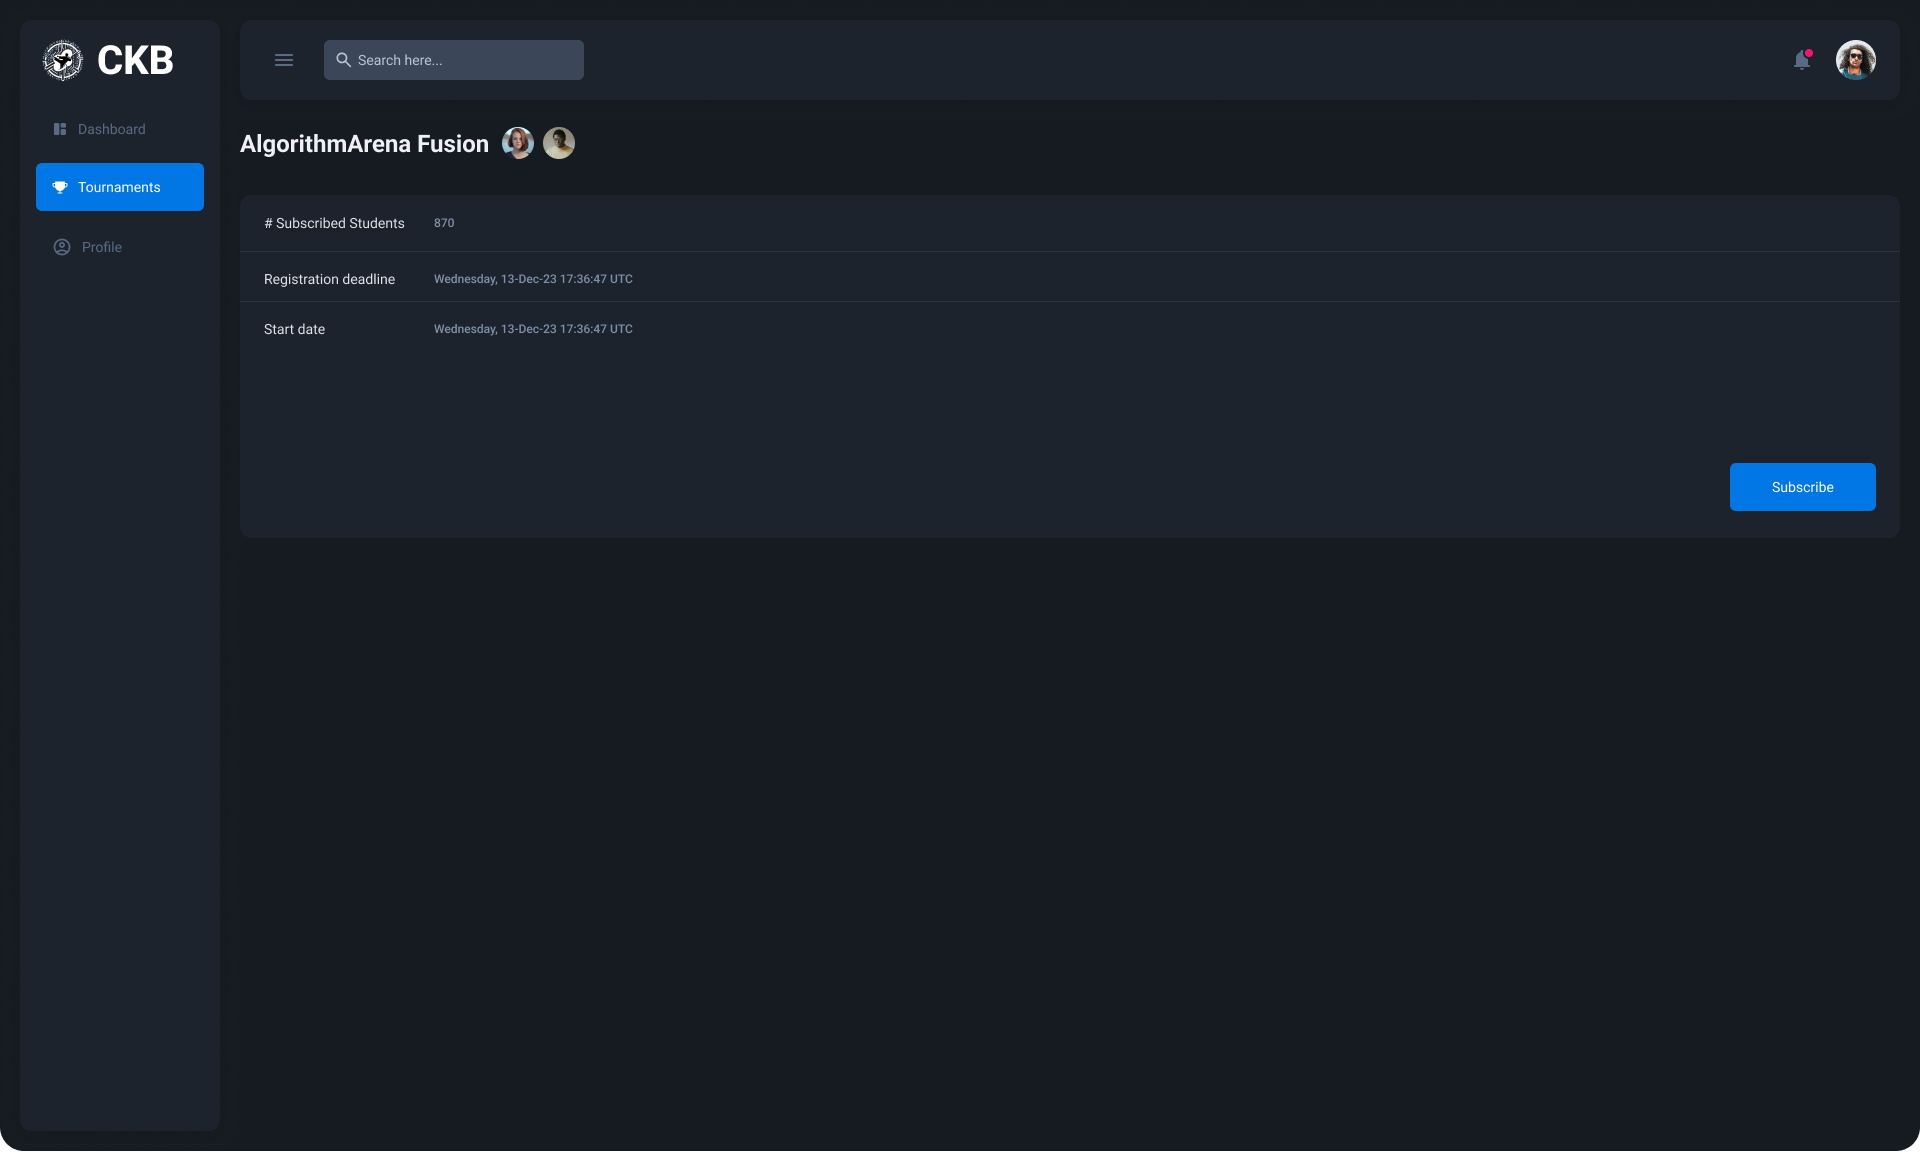
\includegraphics[width=\textwidth]{Images/Dashboard-Tournament-OverView.png}
    \caption{Student Dashboard Tournament OverView}
    \label{fig:student-Tournament-OverView}
\end{figure}

\begin{figure}[H]
    \centering
    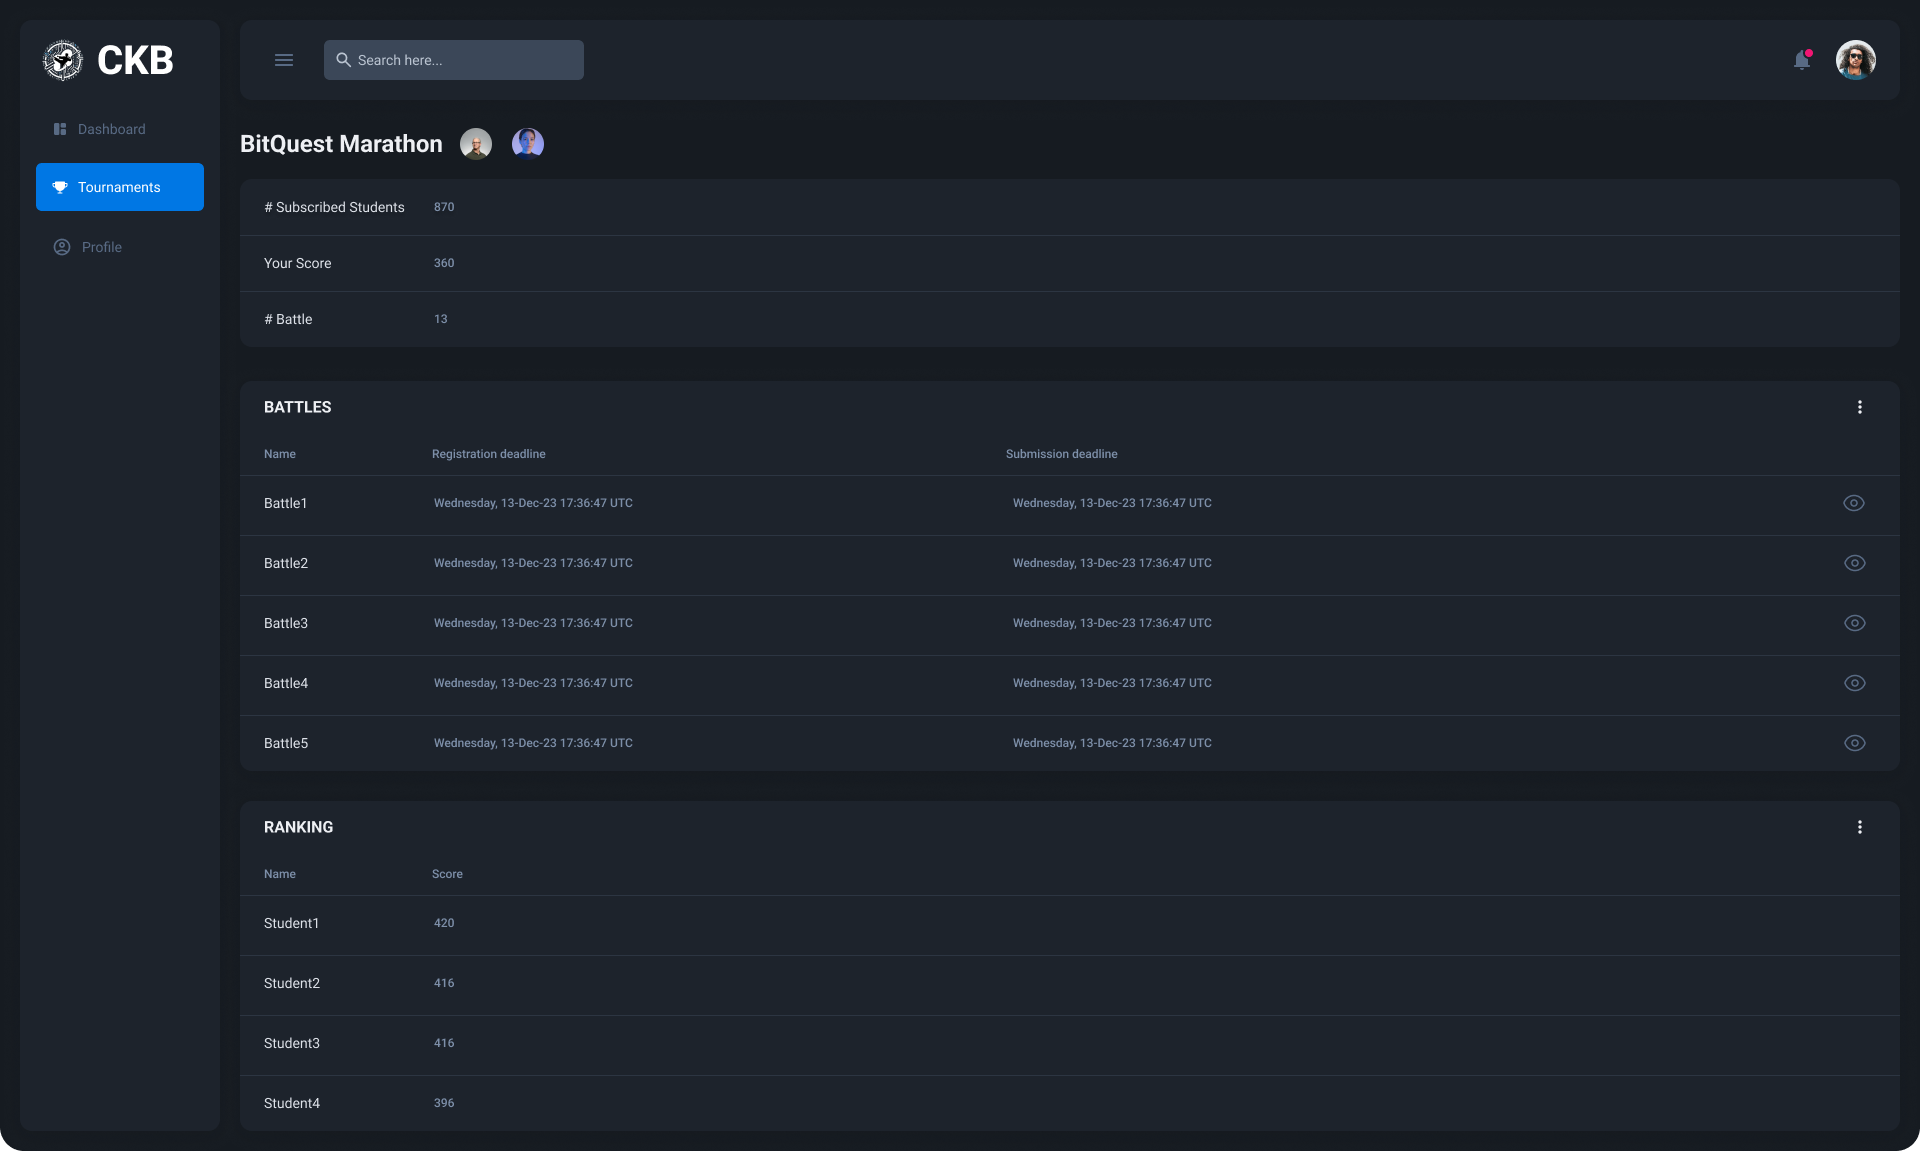
\includegraphics[width=\textwidth]{Images/Dashboard-Tournament-Ongoing.png}
    \caption{Student Dashboard Tournament Ongoing}
    \label{fig:student-Tournament-Ongoing}
\end{figure}

\begin{figure}[H]
    \centering
    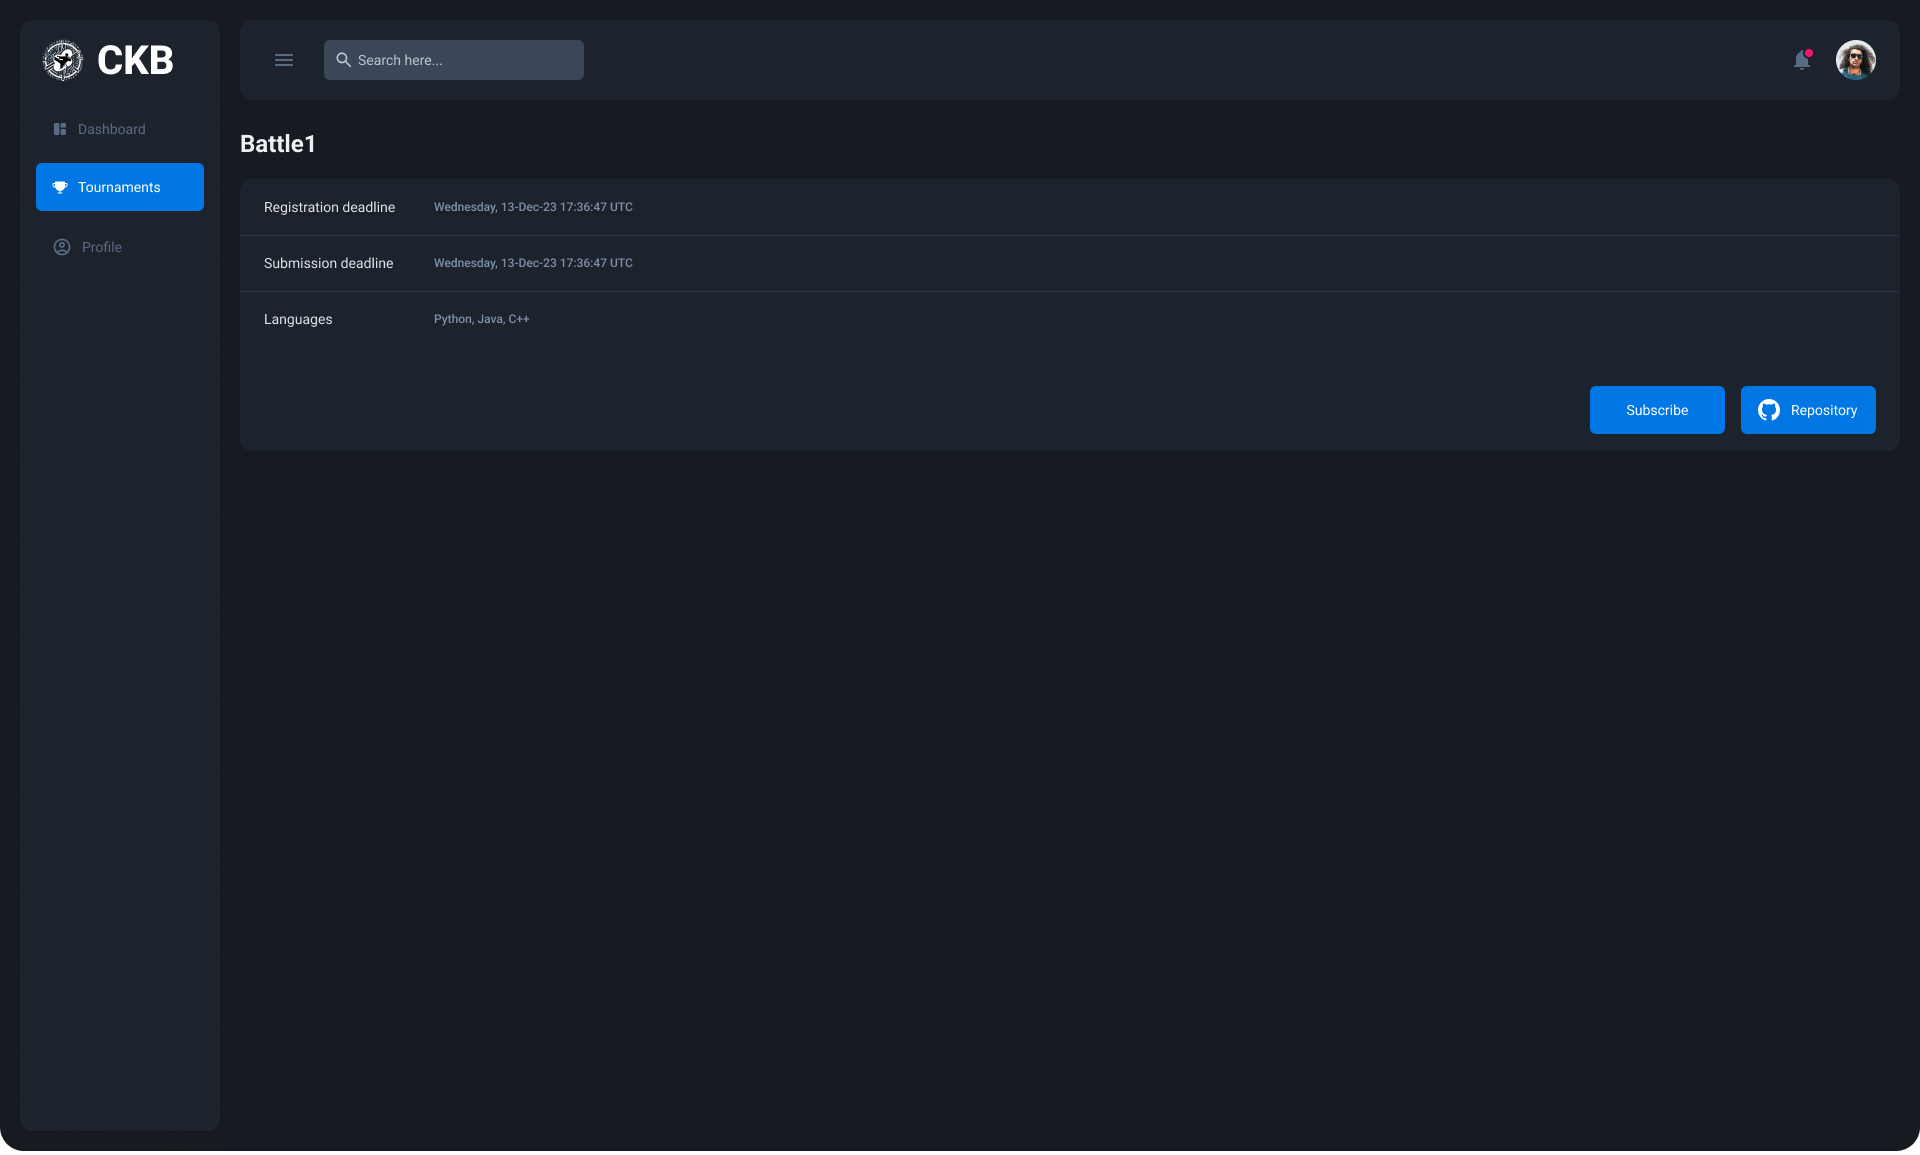
\includegraphics[width=\textwidth]{Images/Dashboard-Battle-Overview.png}
    \caption{Student Dashboard Battle Overview}
    \label{fig:student-Tournament-Completed}
\end{figure}

\begin{figure}[H]
    \centering
    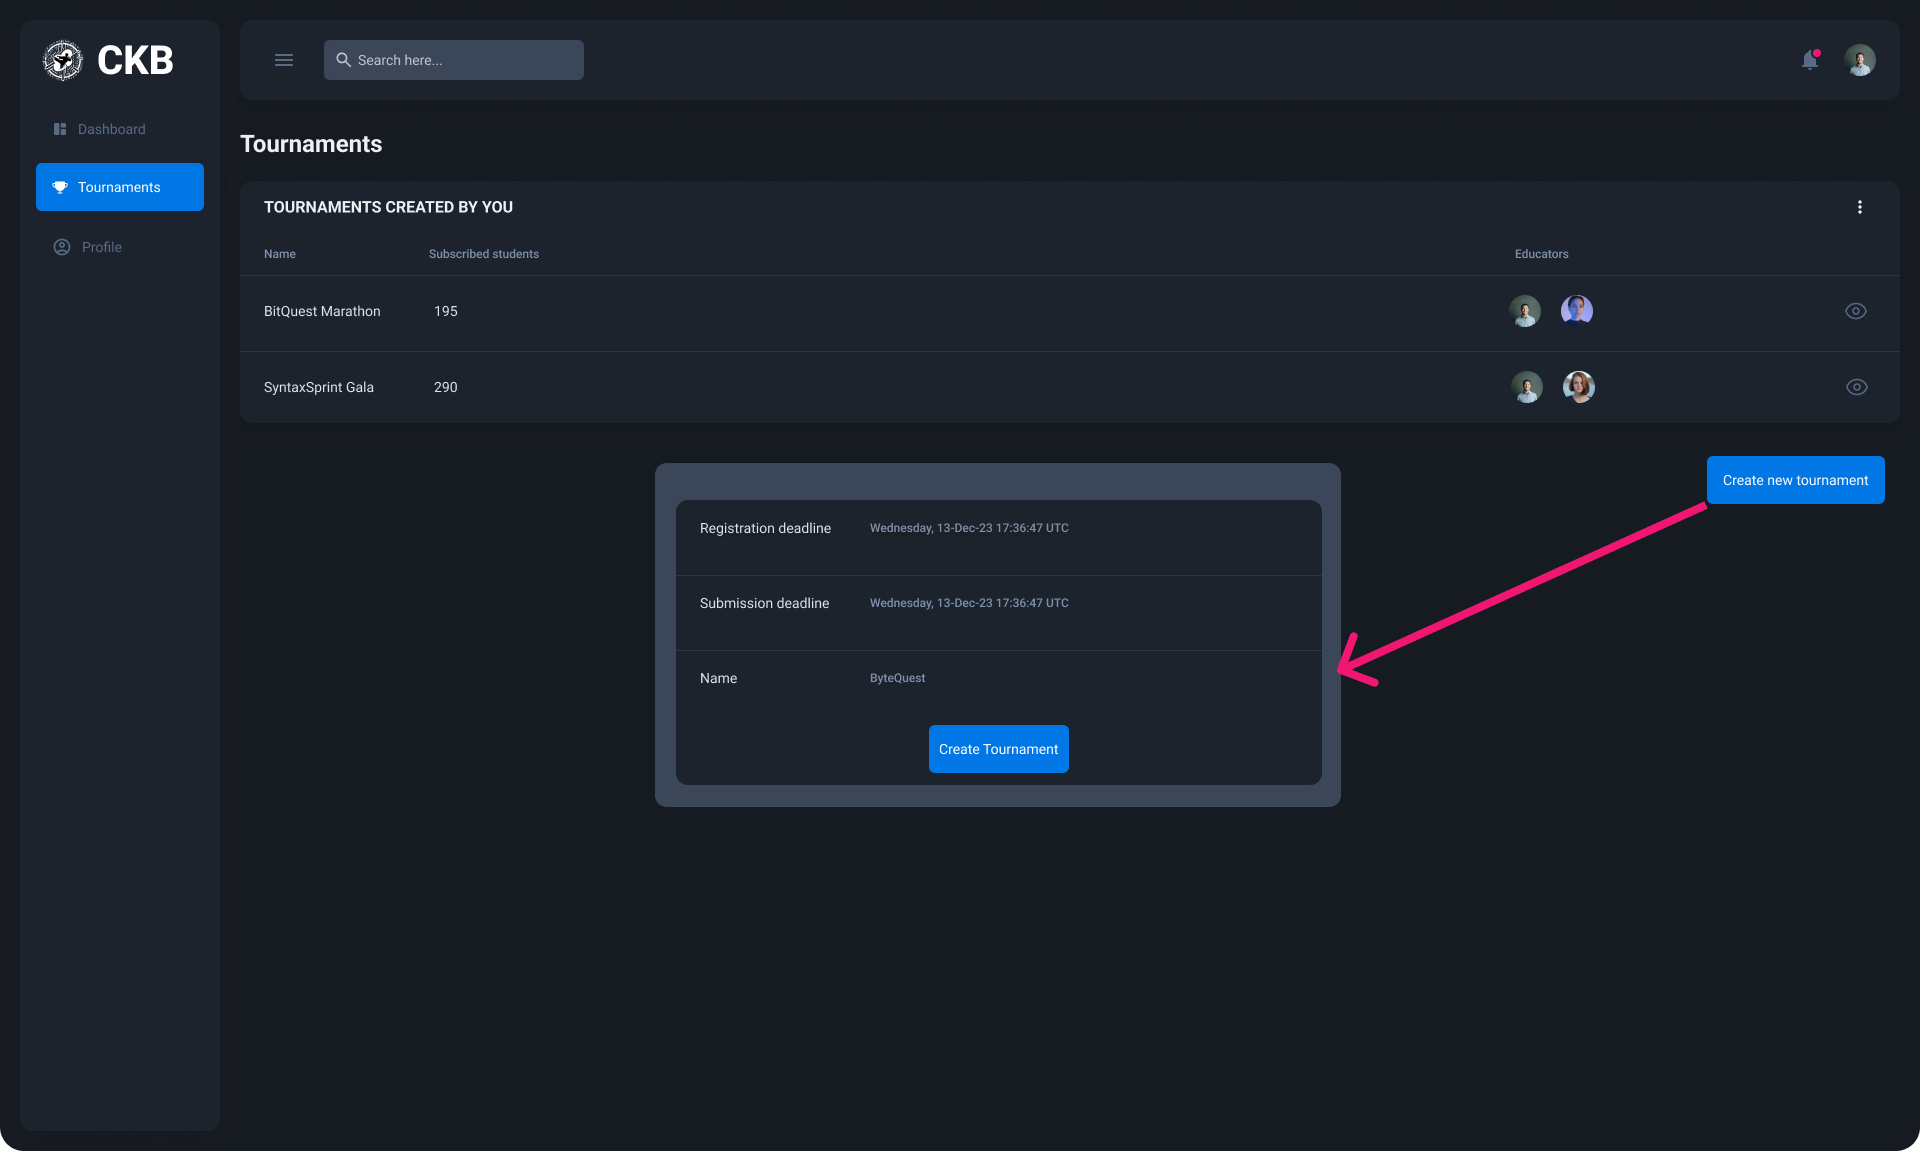
\includegraphics[width=\textwidth]{Images/TournamentCreationEducator.png}
    \caption{Educator Tournament Creation}
    \label{fig:student-Tournament-Completed}
\end{figure}

\begin{figure}[H]
    \centering
    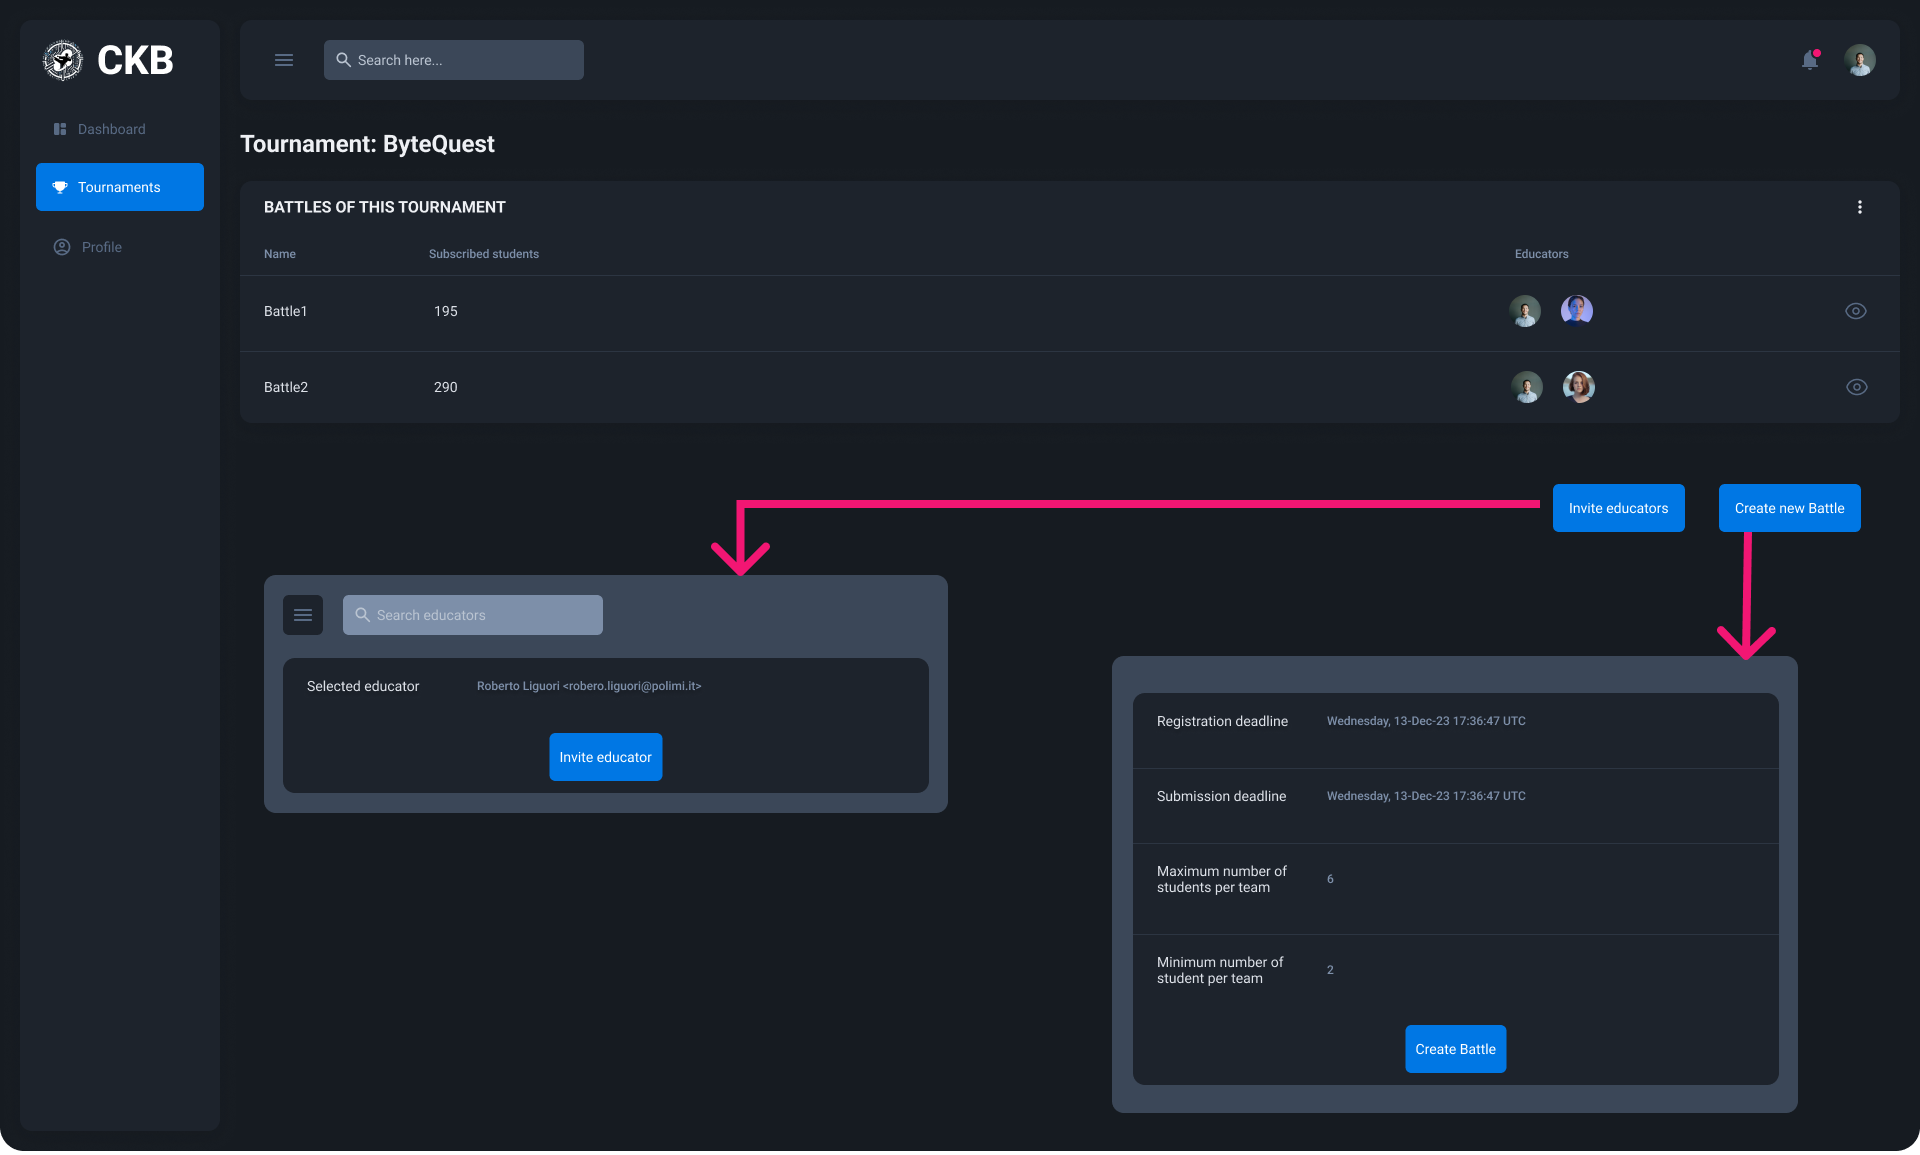
\includegraphics[width=\textwidth]{Images/BattleEducator.png}
    \caption{Educator Battle Creation and Educator invitation}
    \label{fig:student-Tournament-Completed}
\end{figure}

\begin{figure}[H]
    \centering
    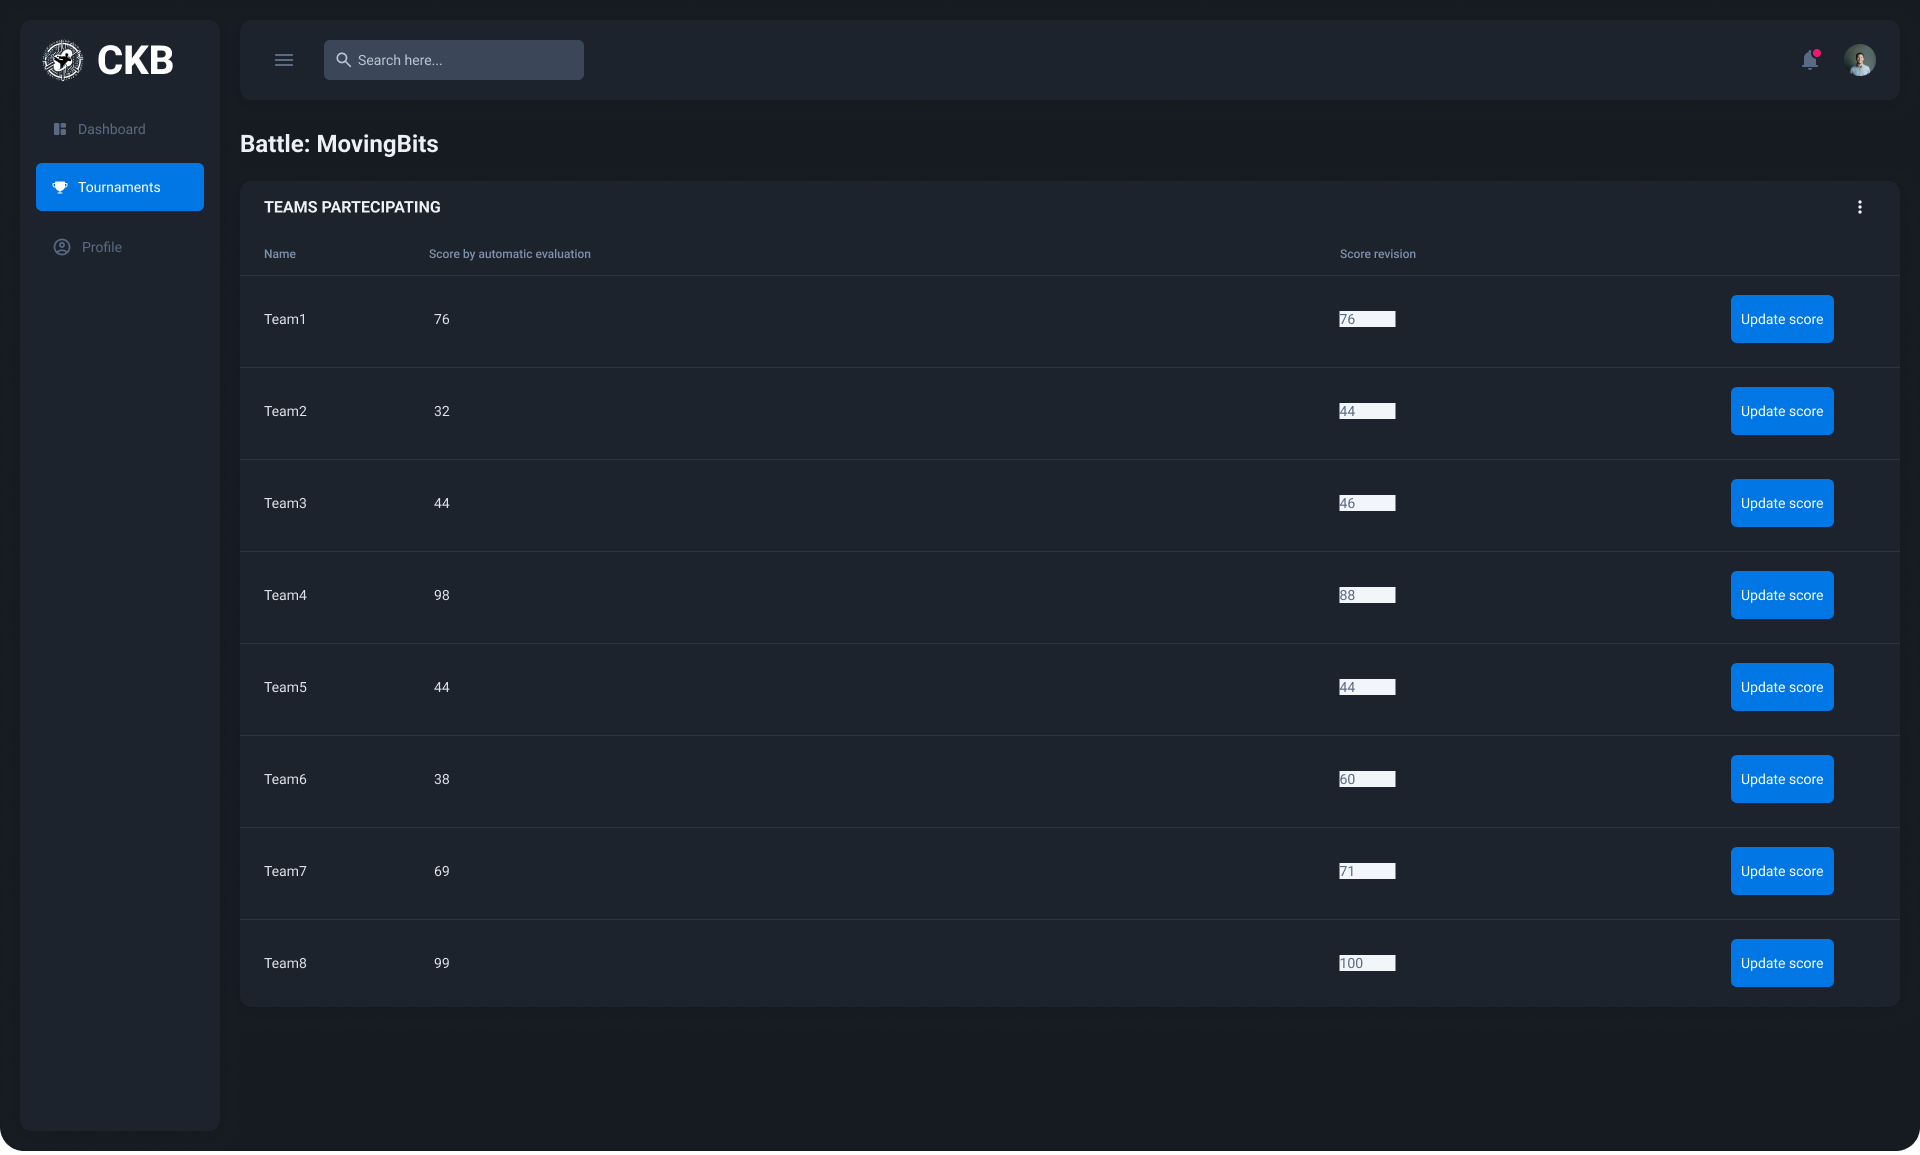
\includegraphics[width=\textwidth]{Images/ManualScoreUpdateEducator.png}
    \caption{Educator Manual Score Update for a battle}
    \label{fig:student-Tournament-Completed}
\end{figure}

%------------------------------------------------------------------------------------------------------------------------------------------------
\clearpage
{\color{Blue}{\section{Requirement Traceability}}}
\label{sect:requirementTraceability}
In this section we will describe the requirements traceability. The requirements traceability is a way to trace the requirements to the design elements. This is done to ensure that all the requirements are met and that the design elements are correct. The requirements traceability is done by using a traceability matrix. The traceability matrix is a table that shows the relationship between the requirements and design elements. \\

\begin{tabular}{|p{3cm}|p{10cm}|}
    \hline
    Requirements & [R1] The system shall allow the user to register to the system \\
    \hline
    Components & 
    \begin{itemize}
        \item RegistrationManager
    \end{itemize} 
    \\
    \hline
\end{tabular}

\begin{tabular}{|p{3cm}|p{10cm}|}
    \hline
    Requirements & [R2] The system shall allow the user to login to the system \\
    \hline
    Components & 
    \begin{itemize}
        \item LoginManager
    \end{itemize} 
    \\
    \hline
\end{tabular}

\begin{tabular}{|p{3cm}|p{10cm}|}
    \hline
    Requirements & [R3] The system shall allow the educator to create a new tournament \\
    \hline
    Components & 
    \begin{itemize}
        \item AuthorizationManager
        \item TournamentManager
    \end{itemize} 
    \\
    \hline
\end{tabular}

\begin{tabular}{|p{3cm}|p{10cm}|}
    \hline
    Requirements & [R4] The system should allow the educator to create a new battle for a tournament \\
    \hline
    Components & 
    \begin{itemize}
        \item AuthorizationManager
        \item TournamentManager
        \item BattleManager
    \end{itemize} 
    \\
    \hline
\end{tabular}

\begin{tabular}{|p{3cm}|p{10cm}|}
    \hline
    Requirements & [R5] The system shall allow the educator to set restriction for a battle \\
    \hline
    Components & 
    \begin{itemize}
        \item AuthorizationManager
        \item BattleManager
    \end{itemize} 
    \\
    \hline
\end{tabular}

\begin{tabular}{|p{3cm}|p{10cm}|}
    \hline
    Requirements & [R6] The system shall allow the educator to upload the CodeKata for a battle \\
    \hline
    Components & 
    \begin{itemize}
        \item AuthorizationManager
        \item BattleManager
        \item CodeKataManager
    \end{itemize} 
    \\
    \hline
\end{tabular}

\begin{tabular}{|p{3cm}|p{10cm}|}
    \hline
    Requirements & [R7] The system shall allow the student to subscribe to a tournament \\
    \hline
    Components & 
    \begin{itemize}
        \item AuthorizationManager
        \item TournamentManager
    \end{itemize} 
    \\
    \hline
\end{tabular}

\begin{tabular}{|p{3cm}|p{10cm}|}
    \hline
    Requirements & [R8] The system shall allow the student to subscribe to a battle \\
    \hline
    Components & 
    \begin{itemize}
        \item AuthorizationManager
        \item BattleMaanger
    \end{itemize} 
    \\
    \hline
\end{tabular}

\begin{tabular}{|p{3cm}|p{10cm}|}
    \hline
    Requirements & [R9] The system shall create a reposistory for each battle such that is forkable by the students \\
    \hline
    Components & 
    \begin{itemize}
        \item BattleManager
        \item GitHub
        \item CodeKataManager
    \end{itemize} 
    \\
    \hline
\end{tabular}

\begin{tabular}{|p{3cm}|p{10cm}|}
    \hline
    Requirements & [R10] The system shall allow the students to create a team for a battle \\
    \hline
    Components & 
    \begin{itemize}
        \item AuthorizationManager
        \item TeamManager
        \item BattleManager
    \end{itemize} 
    \\
    \hline
\end{tabular}

\begin{tabular}{|p{3cm}|p{10cm}|}
    \hline
    Requirements & [R11] The system should allow the students to invite other students to join a team \\
    \hline
    Components & 
    \begin{itemize}
        \item AuthorizationManager
        \item TeamManager
        \item InvitationManager
        \item BattleManager
    \end{itemize} 
    \\
    \hline
\end{tabular}

\begin{tabular}{|p{3cm}|p{10cm}|}
    \hline
    Requirements & [R12] The system should notify students subscribed to the platform when a new tournament is created \\
    \hline
    Components & 
    \begin{itemize}
        \item NotificationManager
    \end{itemize} 
    \\
    \hline
\end{tabular}

\begin{tabular}{|p{3cm}|p{10cm}|}
    \hline
    Requirements & [R13] The system should notify students subscribed to a tournament when a new battle is created \\
    \hline
    Components & 
    \begin{itemize}
        \item NotificationManager
    \end{itemize} 
    \\
    \hline
\end{tabular}

\begin{tabular}{|p{3cm}|p{10cm}|}
    \hline
    Requirements & [R14] The system should notify students subscribed to a tournament when the system puslishes the ranking of the tournament \\
    \hline
    Components & 
    \begin{itemize}
        \item NotificationManager
        \item RankingManager
    \end{itemize} 
    \\
    \hline
\end{tabular}

\begin{tabular}{|p{3cm}|p{10cm}|}
    \hline
    Requirements & [R15] The system shall guarantee that the restrictions for a battle set by the educator are respected \\
    \hline
    Components & 
    \begin{itemize}
        \item BattleManager
    \end{itemize} 
    \\
    \hline
\end{tabular}

\begin{tabular}{|p{3cm}|p{10cm}|}
    \hline
    Requirements & [R16] The system shall allow the educator that created a tournament to invite other educators to the tournament \\
    \hline
    Components & 
    \begin{itemize}
        \item AuthorizationManager
        \item TournamentManager
        \item InvitationManager
    \end{itemize} 
    \\
    \hline
\end{tabular}


\begin{tabular}{|p{3cm}|p{10cm}|}
    \hline
    Requirements & [R17] The system shall allow the educator to close a tournament \\
    \hline
    Components & 
    \begin{itemize}
        \item AuthorizationManager
        \item TournamentManager
    \end{itemize} 
    \\
    \hline
\end{tabular}

\begin{tabular}{|p{3cm}|p{10cm}|}
    \hline
    Requirements & [R18] The system should allow the educator to manually update the score of a team for a battle \\
    \hline
    Components & 
    \begin{itemize}
        \item SubmissionManager
        \item AuthorizationManager
    \end{itemize} 
    \\
    \hline
\end{tabular}

\begin{tabular}{|p{3cm}|p{10cm}|}
    \hline
    Requirements & [R19] The system should allow GitHub to trigger the automatic evaluation of a submission \\
    \hline
    Components & 
    \begin{itemize}
        \item SubmissionManager
        \item EvaluationManager
        \item GitHub
        \item AuthorizationManager
    \end{itemize} 
    \\
    \hline
\end{tabular}
%-------------------------------------------------------------------------------------------------------------------------------------------------

\clearpage
{\color{Blue}{\section{Implementation, Integration and Test Plan}}}
\label{sect:implementationIntegrationTestPlan}
\subsection{Overview}
This section is dedicated to the implementation, integration and test plan. The first part of this section will be dedicated to the identification of the main features of the system and the definition of the components that will be used to implement them. The second part will be dedicated to the integration and testing of the components. The third part will be dedicated to the system testing. The last part will be dedicated to the additional specifications on testing.
\subsubsection{Features identification}
The following list describes the main features of the system and the components that will be used to implement them:
\begin{itemize}
    \item \textbf{User registration and login}: this feature will be implemented by the WebApp and by two componenets that belongs to the Application Server: the RegistrationManager and the LoginManager. The WebApp will provide the user interface for the registration and login process. The RegistrationManager will provide the logic for the registration while the LoginManager will take care of the login process.
    \item \textbf{Creation of a Tournament}: this feature is an educator only feature. It will be implemented by the WebApp to insert the details and restrictions about the tournament, by the AuthorizationManager in order to check if the user is an educator and finally by the TournamentManager. The WebApp will provide the user interface for the creation of a tournament. The TournamentManager will provide the logic for the creation of a tournament.
    \item \textbf{Creation of a Battle}: this feature is an educator only feature. It will be implemented by the WebApp to insert the details and restrictions about the battle, by the AuthorizationManager in order to check if the user is an educator, by the BattleManager and its subcomponent: the CodeKataManager. Finally, since every battle must have their own GitHub repository the BattleManager will also handle the communication with the external system GitHub in order to create the repository for the battle. The WebApp will provide the user interface for the creation of a battle. The CodeKataManager will take care of the creation of the Code Kata while the BattleManager will provide the logic for the creation of a battle.
    \item \textbf{Manage Team}: this feature is a student only feature. It will be implemented by the WebApp to provide the name of the team and also to select the student to invite to the team. The AuthorizationManager will check if the user is a student, the TeamManager will provide the logic for the creation of a team. The BattleManager will be used to associate the newly created team with the battle of interest. The WebApp will provide the user interface for the creation of a team. Additionally the invitiation to join a team is handled by the InvitationManager.
    \item \textbf{Automatic Evaluation}: this feature is one of the most important features of the system. The implementation of this feature will be achieved by the use of the SubmissionManager, EvaluationManager and GitHub. The SubmissionManager will take care of the submission done by the Team on the forked GitHub repository of the battle. The EvaluationManager is responsible for the running of the automatic evaluation on the submitted code. The automatic evaluation starts when the GitHub action set up by the Team is triggered by a push on the forked repository. When the GitHub action is triggered it will call an API endpoint that will start the evaluation process. Finally, there is the RankingMaanger that will take care of the ranking of the students for the battle.
    \item \textbf{Manual Evaluation}: this feature is an educator only feature. It will be implemented by the WebApp to provide the educator with the possibility to manually update the score of an evaluation. The AuthorizationManager will check if the user is an educator. The EvaluationManager is the component that will be used to update the score of an evaluation. Finally, there is the RankingMaanger that will take care of the update of the ranking of the students for the battle.
    \item \textbf{Educator Invitation}: this feature is an educator only feature. It will be implemented by the WebApp to provide the educator with the possibility to invite other educators to join a tournament. The AuthorizationManager will check if the user is an educator. The InvitationManager will take care of the invitation process. Finally the TorunamentManager will be used to associate the invited educator with the tournament if the invitation is accepted.
    \item \textbf{Notification of the user}: the notification feature is trasversal to multiple features. These features are: the creation of a tournament, the creation of a battle, the invitation to join a team, the invitation to join a tournament. The NotificationManager will be used to send the notification to the user. The WebApp will provide the user interface to view the notifications.
\end{itemize}
\subsubsection{Implementation, Integration and Test Plan}
The system is composed by the following subsystems:
\begin{itemize}
    \item \textbf{WebApp}
    \item \textbf{WebServer}
    \item \textbf{Application Server}
    \item \textbf{DBMS}
    \item \textbf{External Services}: GitHub
\end{itemize}
These subsystems are developed, tested, and integrated using a bottom-up approach.
The bottom-up strategy begins at the granular level, focusing on the creation and development of individual components or modules. Each of these elements is designed and developed in isolation, allowing for a deep focus on functionality and performance. This approach ensures that every component is robust and fully operational before it becomes part of a larger system. 

Once these individual modules are developed, they undergo rigorous testing to identify and rectify any issues early in the development cycle. This early detection of problems is a key advantage, as it significantly reduces the complexity and cost of fixes later on. 

After ensuring the reliability of each component, the process moves to the integration phase. Here, these independently developed modules are gradually assembled to form larger subsystems. This step-by-step assembly allows for careful monitoring of interactions between components, ensuring overall system coherence and performance.

Finally, these subsystems are integrated to complete the overall system or project. This incremental approach not only facilitates detailed scrutiny at each stage but also allows for parallel development of components, accelerating the overall timeline. Additionally, it provides flexibility in adapting to changes or incorporating new technologies as development progresses. 

This method emphasizes the significance of various functionalities while aiming to deliver a tangible application feature at each stage of the plan. For each subsystem, we will focus on the implementation, integration, and testing of its constituent components.

It's important to note that components belonging to external systems are not subject to implementation and testing within our plan. These external components are assumed to be reliable and are treated as such.

The following diagrams shows the order in which the components will be implemented, integrated and tested. The arrows represent the dependencies between the components. The components that are not connected by an arrow are independent and can be implemented, integrated and tested in any order.

\subsubsection*{Submission and Evaluation service}
The main components of the Submission and Evaluation service are the SubmissionManager, EvaluationManager, RankingManager and the DBMS Component. The SubmissionManager depends on the EvaluationManager, the RankingManager depends on the EvaluationManager and the DBMS and the the RankingManager depends on the DBMS.
\begin{figure}[H]
    \centering
    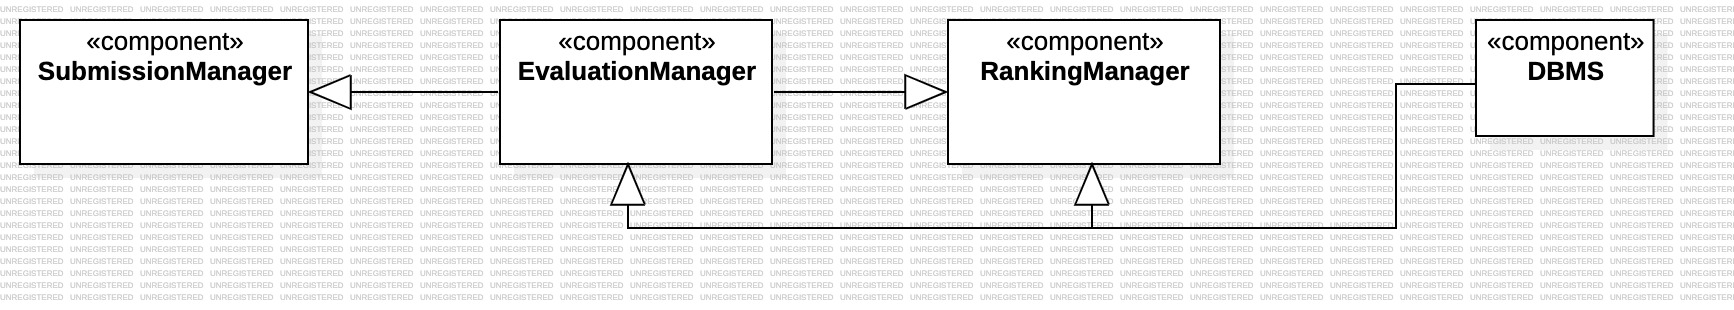
\includegraphics[width=\textwidth]{Diagrams/SubmissionIntegrationPlan.jpg}
    \caption{Submission and Evaluation service}
    \label{fig:submission_and_evaluation}
\end{figure}

\subsubsection*{Notification service}
The main components of the Notification service are the DBMS, the NotificationManager, the TournamentManager, the BattleManager and the InvitationManager. The NotificationManager depends on the DBMS. The TournamentManager, BattleManager and InvitationManager depend on the NotificationManager.
\begin{figure}[H]
    \centering
    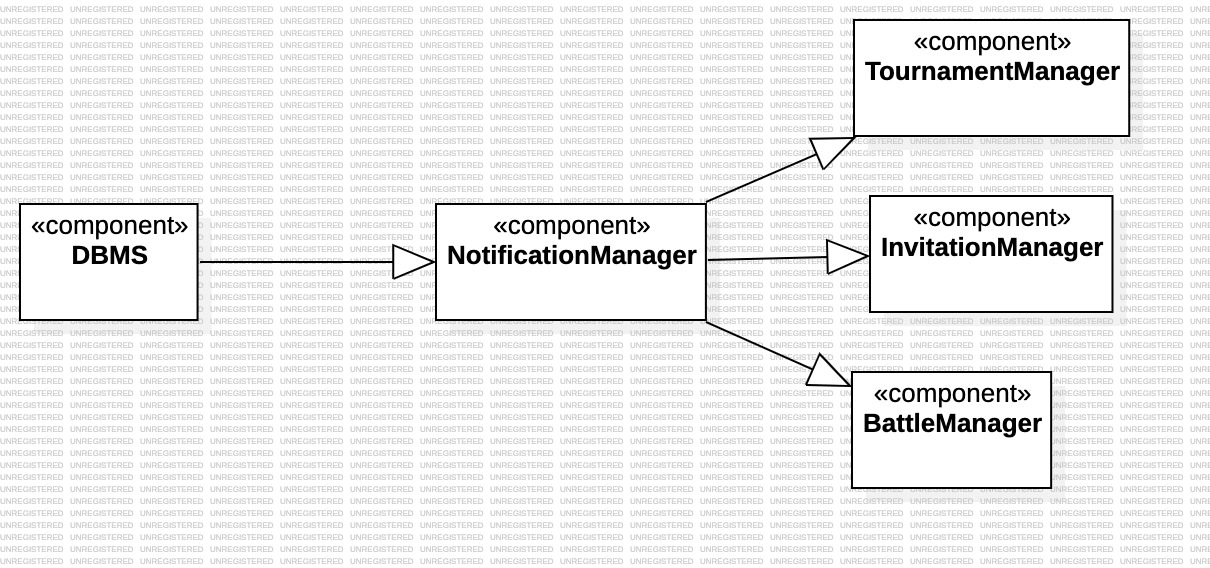
\includegraphics[width=\textwidth]{Diagrams/NotificationIntegrationPlan.jpg}
    \caption{Notification service}
    \label{fig:notification}
\end{figure}

\subsubsection*{Authorization service}
Regarding the Authorization service, the main component is the AuthorizationManager that depends on the TeamManager, the TournamentManager, the BattleManager, the InvitationManager and the EvaluationManager.
\begin{figure}[H]
    \centering
    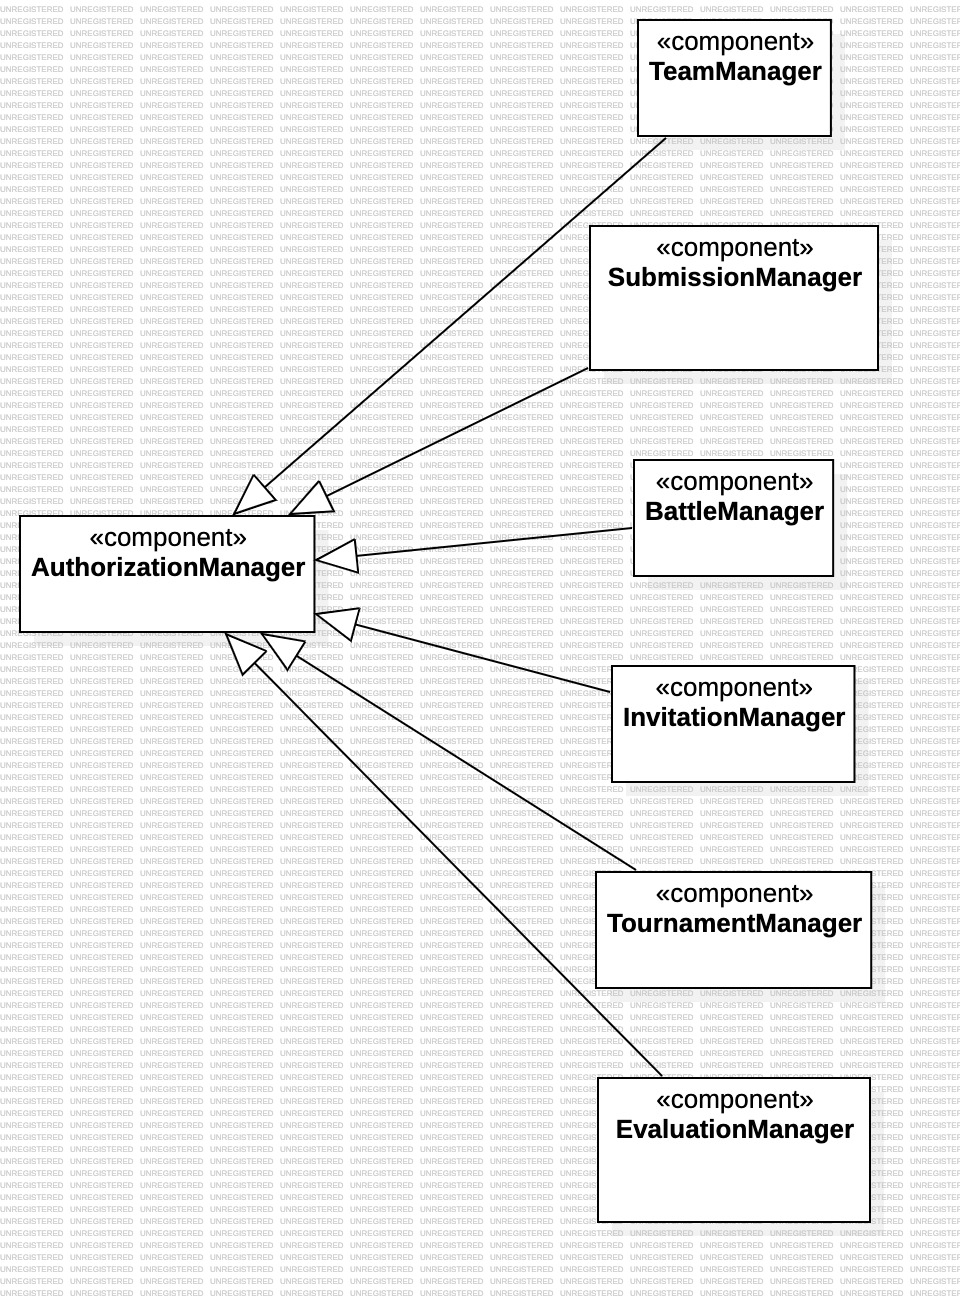
\includegraphics[width=\textwidth]{Diagrams/AuthorizationIntegrationPlan.jpg}
    \caption{Authorization service}
    \label{fig:authorization}
\end{figure}

\subsubsection*{Dispatcher service}
The Dispatcher service is composed by the APIGateway, in order to dispatch the requests to the correct component it needs the AuthorizationManager, LoginManager, RegistrationManager and the RankingManager.
\begin{figure}[H]
    \centering
    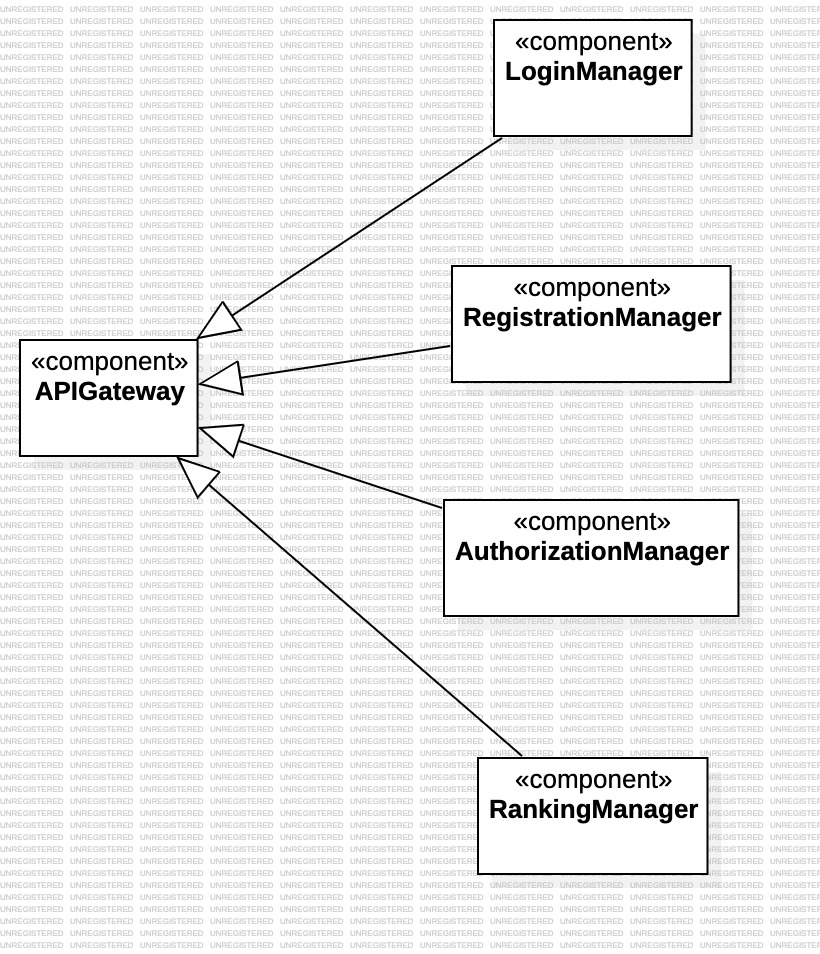
\includegraphics[width=\textwidth]{Diagrams/DispatcherIntegrationPlan.jpg}
    \caption{Dispatcher service}
    \label{fig:dispatcher}
\end{figure}

\subsubsection*{System integration}
The system integration is the last step of the implementation, integration and test plan. The system integration is composed by the integration of the WebApp, WebServer, Application Server and the DBMS. The WebApp depends on the WebServer, the WebServer depends on the Application Server and the Application Server depends on the DBMS. Finally for the external services we have GitHub that depends on the Application Server.
\begin{figure}[H]
    \centering
    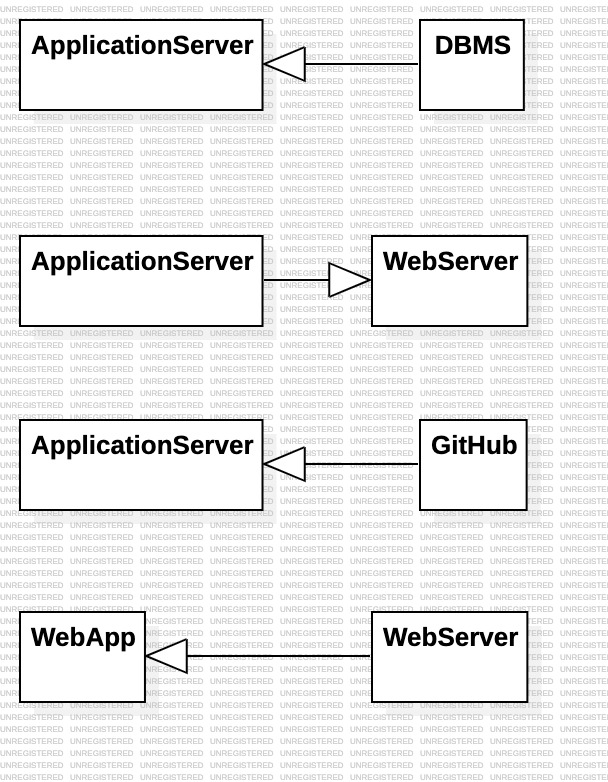
\includegraphics[width=\textwidth]{Diagrams/SystemIntegrationPlan.jpg}
    \caption{System integration}
    \label{fig:system_integration}
\end{figure}
\subsection{System testing}
\subsection{Additional specifications on testing}

%------------------------------------------------------------------------------------------------------------------------------------------------
\clearpage
{\color{Blue}{\section{Effort Spent}}}
\label{sect:effort}
This section provides an estimation of the effort spent by each member of the group to redact this document. The time for each section includes the time spent to write, to discuss and to review the document itself.\\


\subsection*{Picone Paolo}
\begin{tabular}{|p{7cm}|p{7cm}|}
    \hline
    \textbf{Section} & \textbf{Hours}\\
    \hline
    1 & 6\\
    \hline
    2 & 13\\
    \hline
    3 & 23\\
    \hline
    4 & 8\\
    \hline
\end{tabular}


\subsection*{Russo Mario}
\begin{tabular}{|p{7cm}|p{7cm}|}
    \hline
    \textbf{Section} & \textbf{Hours}\\
    \hline
    1 & 6\\
    \hline
    2 & 14\\
    \hline
    3 & 22\\
    \hline
    4 & 8\\
    \hline
\end{tabular}



%------------------------------------------------------------------------------------------------------------------------------------------------
\clearpage
\addcontentsline{toc}{section}{References}
\bibliographystyle{plain}
\bibliography{main}
\begin{itemize}
        \item Document written using \LaTeX  \ and Visual Studio Code
        \item Diagrams created using StarUML 6.0.1
        \item Mockups created using Figma
\end{itemize}
%------------------------------------------------------------------------------------------------------------------------------------------------
\end{document}
